\documentclass[12pt]{article}

% Better font shapes (fixes \textbackslash in \texttt)
\usepackage[T1]{fontenc}
\usepackage{lmodern}

% Core math
\usepackage{amsmath, amssymb, amsthm}
\usepackage{mathpartir}

% Diagrams
\usepackage{tikz-cd}
\usepackage{tikz}
\usetikzlibrary{arrows.meta, positioning, shapes.geometric, fit, backgrounds}

% References
\usepackage{hyperref}
\usepackage{xurl}    % aggressive URL line-breaking, helps bib entries
\usepackage{cleveref}

% Graphics
\usepackage{graphicx}

% Page layout
\usepackage[margin=1in]{geometry}

% Listings for Rust code
\usepackage{listings}
\usepackage{xcolor}

% GrokRxiv sidebar uses LaTeX kernel shipout hook (everypage was legacy)

% Header/spacing
\usepackage{enumitem}

% Theorem environments
\newtheorem{theorem}{Theorem}[section]
\newtheorem{proposition}[theorem]{Proposition}
\newtheorem{lemma}[theorem]{Lemma}
\newtheorem{corollary}[theorem]{Corollary}
\theoremstyle{definition}
\newtheorem{definition}[theorem]{Definition}
\theoremstyle{remark}
\newtheorem{remark}[theorem]{Remark}
\newtheorem*{example}{Example}

% --- Custom math commands -------------------------------------------------
\newcommand{\lifetime}[1]{\ensuremath{\,'\!#1}}
\newcommand{\borrow}[2]{\ensuremath{\&^{#1}\,#2}}
\newcommand{\mutborrow}[1]{\ensuremath{\&\mathsf{mut}\;#1}}
\newcommand{\owned}[1]{\ensuremath{\mathsf{Box}\langle #1\rangle}}
\newcommand{\Result}[2]{\ensuremath{\mathsf{Result}\langle #1,\,#2\rangle}}
\newcommand{\Option}[1]{\ensuremath{\mathsf{Option}\langle #1\rangle}}
\newcommand{\Vecc}[1]{\ensuremath{\mathsf{Vec}\langle #1\rangle}}
\newcommand{\VecDeque}[1]{\ensuremath{\mathsf{VecDeque}\langle #1\rangle}}
\newcommand{\Slice}[1]{\ensuremath{[\,#1\,]}}
\newcommand{\region}[1]{\ensuremath{\rho_{#1}}}
\newcommand{\subtype}{\ensuremath{<:}}
\newcommand{\outlives}{\ensuremath{:}}
\newcommand{\judg}[3]{\ensuremath{#1 \vdash #2 : #3}}

% --- Listings: Rust style -------------------------------------------------
\definecolor{rustkw}{RGB}{170,34,140}
\definecolor{rusttype}{RGB}{0,90,156}
\definecolor{ruststring}{RGB}{0,128,0}
\definecolor{rustcomment}{RGB}{120,120,120}
\definecolor{rustbg}{RGB}{248,248,248}

\lstdefinelanguage{Rust}{
  morekeywords={fn,let,mut,pub,struct,enum,impl,trait,for,where,if,else,match,return,
                use,mod,crate,self,Self,as,in,loop,while,break,continue,move,ref,
                unsafe,extern,async,await,dyn,box,type,const,static,super,
                true,false,None,Some,Ok,Err},
  morekeywords=[2]{u8,u16,u32,u64,usize,i8,i16,i32,i64,isize,bool,char,str,String,
                   Vec,VecDeque,Option,Result,Box,Rc,Arc,Cow,HashMap,BTreeMap,
                   Read,Write,Iterator},
  sensitive=true,
  morecomment=[l]{//},
  morecomment=[s]{/*}{*/},
  morestring=[b]",
}

\lstset{
  language=Rust,
  basicstyle=\ttfamily\small,
  keywordstyle=\color{rustkw}\bfseries,
  keywordstyle=[2]\color{rusttype},
  commentstyle=\color{rustcomment}\itshape,
  stringstyle=\color{ruststring},
  backgroundcolor=\color{rustbg},
  frame=single,
  framerule=0pt,
  rulecolor=\color{rustbg},
  numbers=none,
  showstringspaces=false,
  breaklines=true,
  columns=fullflexible,
  xleftmargin=8pt,
  xrightmargin=4pt,
  aboveskip=8pt,
  belowskip=8pt,
}

% --- GrokRxiv sidebar -----------------------------------------------------
\definecolor{grokgray}{RGB}{110,110,110}
\AddToHook{shipout/foreground}{%
  \ifnum\value{page}=1
    \begin{tikzpicture}[remember picture, overlay]
      \node[
        rotate=90,
        anchor=south,
        font=\Large\sffamily\bfseries\color{grokgray},
        inner sep=0pt
      ] at ([xshift=38pt, yshift=0.52\paperheight]current page.south west)
      {GrokRxiv:2026.04.rust\quad
       [\,cs.PL\,]\quad
       16 Apr 2026};
    \end{tikzpicture}
  \fi
}

\title{Idiomatic Safe Rust as a Translation Target:\\
Ownership, Lifetimes, and ABI-Compatible Parser Design\\
{\large A Case Study in \texttt{safe-libyaml}}}

\author{Matthew Long \\
\textit{The YonedaAI Collaboration, YonedaAI Research Collective} \\
Chicago, IL \\
\texttt{matthew@yonedaai.com} $\cdot$ \url{https://yonedaai.com}}

\date{April 16, 2026}

\begin{document}
\maketitle

\begin{abstract}
The migration of legacy C libraries to Rust is bottlenecked less by syntax than
by the inverse problem of \emph{recovering} the implicit invariants that C never
forced its programmers to state. This paper is a \emph{design specification}:
it characterises the \emph{target} side of that recovery by enumerating, in
concrete and reviewable form, what idiomatic safe Rust should look like for
a streaming parser library, and what engineering rules a translation pipeline
must follow to hit that target deterministically.
We do \emph{not} report performance numbers for an existing automated port;
the proposed crate \texttt{safe-libyaml} is in-progress and the figures we
cite (e.g.\ ``parity with C'') are inherited from S.~Ask's \emph{manual}
port \texttt{libyaml-safer} and stated explicitly as engineering targets,
not measurements. The contribution is a systems-engineering specification
plus the agent-level build plan needed to realise it.
We adopt a deliberately lightweight notation for lifetime subtyping
($\lifetime{a} \outlives \lifetime{b}$), the borrow judgment
$\judg{\Gamma}{e}{\tau\langle\rho\rangle}$, and the
\texttt{Result}/\texttt{Option} algebra (Section~\ref{sec:framework}). The
notation is a \emph{clarity tool}: it lets us state precisely which
components of the design are forced by Rust's type system and which are
engineering choices. We do not claim any new formal result about Rust
itself; the soundness theorems we cite are RustBelt's~\cite{rustbelt}.
The substantive contributions are: (i) a lifetime-parameterised
\texttt{Event<\lifetime{a}>} enum with \texttt{Cow<\lifetime{a}, str>}
payloads (Section~\ref{sec:lifetimes-events}); (ii) a
\texttt{thiserror}-derived structured error matching libyaml's existing
problem categories (Section~\ref{sec:errors}); (iii) the
\texttt{Vec}/\texttt{VecDeque} mapping for libyaml's
\texttt{STACK\_*}/\texttt{QUEUE\_*} macro family (Section~\ref{sec:memory});
and (iv) a strict no-\texttt{unsafe} core paired with a thin
\texttt{extern "C"} ABI shim \texttt{safe-libyaml-sys}
(Sections~\ref{sec:unsafe}--\ref{sec:ffi}) that preserves the exact symbol
set required by existing C callers and by Rust crates such as
\texttt{serde\_yaml\_ng} and \texttt{serde\_yaml\_bw}. Appendix~A is
supplementary material: a 32-task agent-level build plan (a detailed,
automatable task list for the prototype-building agents that the project's
pipeline executes) that demonstrates \emph{implementability} of the design
but is not itself a research result.
The paper is self-contained; references to other papers in the
\emph{Ferrous Bridge} project~\cite{long-c, long-transpile,
long-c2rust-strategy} are pointers, not prerequisites.
\end{abstract}

\tableofcontents
\newpage

% =========================================================================
\section{Introduction}
\label{sec:intro}

\subsection{What ``safe and idiomatic'' means in this paper}

Rust's marketing surface\,---\,``a systems language without the segfaults''\,---\,
underdetermines what ``safe'' means as an engineering target. We take three
operational definitions throughout the paper.

\begin{definition}[Safe Rust]
\label{def:safe-rust}
A Rust crate is \emph{safe} if it contains no \texttt{unsafe} blocks outside of
a thin, separately-versioned FFI boundary, and if its entire test suite passes
under \emph{Miri}~\cite{miri-popl2026} with zero undefined behaviour reports
under the Stacked Borrows aliasing model.
\end{definition}

\begin{definition}[Idiomatic Rust]
\label{def:idiomatic-rust}
A Rust crate is \emph{idiomatic} if it (i) replaces every C-style integer error
return with a \texttt{Result<T,E>}; (ii) replaces every nullable pointer with
\texttt{Option<T>}; (iii) replaces every tagged union with an \texttt{enum}
whose exhaustiveness is checked by the compiler; (iv) prefers iterator
adaptors over manual index loops; and (v) passes \verb|cargo clippy -- -W clippy::pedantic|
with no allowed lints other than those documented
in the crate's lint policy.
\end{definition}

\begin{definition}[ABI-compatible]
\label{def:abi-compat}
A Rust crate is \emph{ABI-compatible} with a C library $L$ if it exports a set
of \texttt{extern "C"} functions whose names, calling conventions, and
\texttt{\#[repr(C)]} struct layouts match $L$'s public header file byte-for-byte
as detected by \texttt{cbindgen} diff and by \texttt{nm} symbol enumeration.
\end{definition}

The thesis of the paper is a \emph{specification} thesis: all three properties
should be simultaneously achievable for a non-trivial streaming parser, and
the engineering rules that would make them achievable can be encoded as
agent prompts and CI gates. We propose those rules concretely; the empirical
verification that the in-progress \texttt{safe-libyaml} actually achieves
them at parity with the C reference is the responsibility of the
companion verification work and is not claimed here as a result.

\subsection{\texttt{safe-libyaml} as the running example}

The \texttt{libyaml} C library is a streaming YAML 1.1 parser/emitter of
roughly 9{,}300 lines of source spread across ten files. The
\texttt{unsafe-libyaml} crate\footnote{\url{https://github.com/dtolnay/unsafe-libyaml}}
is a mechanical \texttt{c2rust} transpilation that retains the original C
control flow but expresses it in pervasively-\texttt{unsafe} Rust; it has
$\approx 90$M cumulative downloads as the parser backend of
\texttt{serde\_yaml}, \texttt{serde\_yaml\_ng}, \texttt{serde\_yaml\_bw}, and
\texttt{serde\_norway}. The \texttt{libyaml-safer}
crate\footnote{\url{https://github.com/simonask/libyaml-safer}} is a one-week
manual safe port by S.\ Ask that demonstrates the exercise is feasible by a
skilled human, and which we use as a quality and performance reference. Our
target crate \texttt{safe-libyaml} is the planned \emph{automated} safe
port produced by the \emph{Ferrous Bridge} pipeline; this paper specifies
its API surface and its agent build plan, but does not report measured
properties of an implementation that does not yet exist. Numbers attributed
to \texttt{libyaml-safer} are external results we cite; numbers attributed
to \texttt{safe-libyaml} are explicit \emph{targets} for the in-progress
build.

\subsection{Outline}

Section~\ref{sec:framework} fixes notation (lifetime regions, the borrow
judgment, the \texttt{Result}/\texttt{Option} algebra) as a clarity tool;
it is not a new formal system.
Section~\ref{sec:ownership-streaming} treats ownership and borrowing for
streaming parsers; Section~\ref{sec:lifetimes-events} dives into the
lifetime-parameterised \texttt{Event<\lifetime{a}>} enum, the central design
decision. Section~\ref{sec:errors} addresses error handling;
Section~\ref{sec:memory} maps libyaml's STACK/QUEUE/STRING macros to safe
\texttt{std} types. Section~\ref{sec:nostd} discusses \texttt{no\_std + alloc}.
Section~\ref{sec:tagged-enums} treats tagged unions vs.\ \texttt{enum}.
Section~\ref{sec:unsafe} formalises the \texttt{unsafe} discipline.
Section~\ref{sec:ffi} specifies the \texttt{\#[repr(C)]} ABI shim and
\texttt{cbindgen} integration. Section~\ref{sec:tooling} surveys the
quality-gate tools. Section~\ref{sec:related} situates the work alongside
\texttt{nom}, \texttt{winnow}, \texttt{rustls}, \texttt{rav1d}, and others.
Section~\ref{sec:results} states the safety results and Section~\ref{sec:disc}
discusses limitations. Section~\ref{sec:concl} concludes.
Appendix~A is the mandatory \emph{Development Plan for Prototype Agents}
covering the scaffold and idiom phase.

% =========================================================================
\section{Notation: A Lightweight Framework}
\label{sec:framework}

\noindent\textit{What this section is and is not.} The fragment of formalism
introduced below is a \emph{notational tool}: it lets later sections state
precisely which parts of the design are forced by Rust's type system and
which are engineering choices. We do not introduce any new formal system,
nor do we prove any new property of Rust itself. Where Rust's full type
system has been formalised --- most completely by the RustBelt
project~\cite{rustbelt} --- we cite their results rather than re-derive
them. The notation is inspired by region-based memory
management~\cite{tofte-talpin} and is adequate for the API-design
statements that follow.

\subsection{Lifetimes as regions}

\begin{definition}[Region]
A \emph{region} (or \emph{lifetime}) $\rho \in \mathcal{R}$ is an element of a
partially-ordered set $(\mathcal{R}, \outlives)$ where $\rho_1 \outlives \rho_2$
(read ``$\rho_1$ outlives $\rho_2$'') means every program point at which a
borrow with lifetime $\rho_2$ is live is dominated by a program point at which
a borrow with lifetime $\rho_1$ is live. The Rust surface syntax writes
$\lifetime{a} \outlives \lifetime{b}$.
\end{definition}

\begin{remark}[Asymmetry of the colon]
The Rust syntax overloads ``\,:\,'' between type ascription
($x : \tau$) and lifetime constraints ($\lifetime{a} : \lifetime{b}$). We
write \,$\outlives$\, for the latter throughout to avoid ambiguity.
\end{remark}

\begin{definition}[Static region]
The distinguished region $\lifetime{static} \in \mathcal{R}$ satisfies
$\lifetime{static} \outlives \rho$ for every $\rho \in \mathcal{R}$. Values of
type $\borrow{\lifetime{static}}{T}$ are valid for the entire program execution.
\end{definition}

\subsection{The borrow judgment}

\begin{definition}[Typing context]
A typing context $\Gamma$ is a finite map from variables to pairs
$(\tau, \rho)$ where $\tau$ is a Rust type and $\rho$ is the region during
which the binding is live. We write $\Gamma, x : \tau \langle \rho \rangle$
for the extension.
\end{definition}

The borrow checker can be presented as a judgment
$\judg{\Gamma}{e}{\tau \langle \rho \rangle}$, read ``in context $\Gamma$,
expression $e$ has type $\tau$ valid in region $\rho$''. Three rules suffice
for our purposes. \emph{Notational bridge:} the formal $\borrow{\rho}{T}$
in this section corresponds to Rust's surface syntax \texttt{\&\lifetime{a}\,T}
(reading $\rho$ as $\lifetime{a}$); $\mutborrow{T}$ corresponds to
\texttt{\&\lifetime{a}\,mut\,T}. The remainder of the paper uses the Rust
surface syntax exclusively; the formal notation appears only in this
section and in the proofs of Propositions~\ref{prop:contravariance},
\ref{prop:cow-events}, and \ref{prop:compositional-safety}.

\begin{mathpar}
\inferrule*[lab=Var]
  { (x : \tau \langle \rho \rangle) \in \Gamma }
  { \judg{\Gamma}{x}{\tau \langle \rho \rangle} }

\inferrule*[lab=Borrow]
  { \judg{\Gamma}{e}{\tau \langle \rho \rangle} \\ \rho' \outlives \rho }
  { \judg{\Gamma}{\&\, e}{\borrow{\rho'}{\tau} \langle \rho' \rangle} }

\inferrule*[lab=Sub]
  { \judg{\Gamma}{e}{\tau \langle \rho \rangle} \\ \rho \outlives \rho' }
  { \judg{\Gamma}{e}{\tau \langle \rho' \rangle} }
\end{mathpar}

\begin{proposition}[Variance of borrow types]
\label{prop:contravariance}
\emph{Shared} borrows are \emph{covariant} in their lifetime parameter:
if $\rho_1 \outlives \rho_2$ then $\borrow{\rho_1}{\tau} \subtype \borrow{\rho_2}{\tau}$.
\emph{Mutable} borrows are \emph{invariant} in their lifetime parameter: if
$\borrow{\rho_1}{\mathsf{mut}\, \tau} \subtype \borrow{\rho_2}{\mathsf{mut}\, \tau}$
then $\rho_1 = \rho_2$. The invariance of the mutable case arises because
$\&\mathsf{mut}\,\tau$ supports both reads (which would justify covariance)
\emph{and} writes (which, symmetrically, would justify contravariance);
the conjunction of covariance and contravariance is invariance.
\end{proposition}

\begin{proof}[Proof sketch]
Subtype substitution must preserve typing in every position. For shared
borrows, only the read position is exercised; a longer lifetime always
admits the uses a shorter one would, hence covariance. For mutable borrows,
the same reasoning gives covariance for the read position but
contravariance for the write position: a write through a long-lived
alias must be visible through every other alias of the same cell, so
shrinking the lifetime in a write-reachable position is unsound. The
conjunction of the two forces invariance. The full argument is RustBelt's
main soundness theorem~\cite{rustbelt}.
\end{proof}

\subsection{The Result and Option algebra}

\begin{definition}[Sum-type error algebra]
For Rust types $T, E$ we have the sum types
\[
\Result{T}{E} \;=\; \mathsf{Ok}(T) + \mathsf{Err}(E),
\qquad
\Option{T} \;=\; \mathsf{Some}(T) + \mathsf{None}.
\]
The \,\texttt{?}\, operator implements the Kleisli composition
$f \;\texttt{?}\; g : \Result{T}{E} \to \Result{U}{E}$, lifting
\,$g : T \to \Result{U}{E}$ across the error monad and short-circuiting on
$\mathsf{Err}$.
\end{definition}

\begin{proposition}[Errors compose via \texttt{?}]
\label{thm:errors-compose}
Let $f_1 : A \to \Result{B}{E_1}$ and $f_2 : B \to \Result{C}{E_2}$. If
the crate's error type $E$ satisfies both $\mathsf{From}\langle E_1\rangle$
and $\mathsf{From}\langle E_2\rangle$, then the composition $f_2 \circ f_1$
has a canonical lift to $A \to \Result{C}{E}$ via the \,\texttt{?}\, operator
alone:
\begin{lstlisting}
fn compose(a: A) -> Result<C, E> {
    let b = f1(a)?;          // ? invokes E::from(E1)
    let c = f2(b)?;          // ? invokes E::from(E2)
    Ok(c)
}
\end{lstlisting}
The \,\texttt{?}\, operator desugars to a match that invokes
\texttt{E::from(e1)} (resp.\ \texttt{E::from(e2)}) on the \texttt{Err}
branch, giving the uniform short-circuit on the error monad.
\end{proposition}

This is the formal justification for the \texttt{thiserror} pattern
discussed in Section~\ref{sec:errors}: deriving \texttt{\#[from]} on each
nested error arm installs the required \texttt{From} instance.

% =========================================================================
\section{Ownership and Borrowing for Streaming Parsers}
\label{sec:ownership-streaming}

A streaming parser sits at the intersection of three resource concerns: an
\emph{input buffer} that someone must own, an emitted \emph{event stream} that
must be either owned or borrowed back into the buffer, and an \emph{internal
state} (token queue, indent stack, mark stack) that is exclusively the
parser's. The C \texttt{libyaml} answer is to make every pointer raw;
the safe-Rust answer is to assign each concern to exactly one of the four
ownership classes.

\begin{definition}[Pointer ownership classification]
\label{def:ownership-class}
For each C pointer $p$ in a function we assign one of:
\begin{itemize}[leftmargin=2em]
\item \textsf{Owning}: $p$ is allocated in the function and freed in the
function (or returned to a caller who is responsible for freeing it).
Rust target: $\owned{T}$ or owned $\Vecc{T}$.
\item \textsf{BorrowShared}: $p$ is read but never written through and
never freed.
Rust target: $\borrow{\lifetime{a}}{T}$ or $\borrow{\lifetime{a}}{\Slice{T}}$.
\item \textsf{BorrowMut}: $p$ is written through but not freed.
Rust target: $\mutborrow{T}$ or $\mutborrow{\Slice{T}}$.
\item \textsf{SharedOwnership}: $p$ is held by multiple owners with potentially
overlapping lifetimes; Rust target: $\mathsf{Rc}\langle T\rangle$ or
$\mathsf{Arc}\langle T\rangle$.
\end{itemize}
\end{definition}

For \texttt{libyaml}'s parser, the classification falls out cleanly: the input
buffer is owned by the \texttt{Parser}; the token queue and the indent and
mark stacks are owned by the \texttt{Parser}; the events emitted to the
caller are either \emph{borrowed} from the buffer
(zero-copy, lifetime-parameterised), or \emph{owned} (allocated string copies).
This dichotomy is the central design tension addressed in
Section~\ref{sec:lifetimes-events}.

\subsection{The single-owner buffer}

The C \texttt{yaml\_parser\_set\_input\_string(parser, input, length)} accepts
a $(\texttt{ptr},\texttt{len})$ pair without specifying ownership. The Rust
analogue must choose. We propose three constructors:

\begin{lstlisting}
impl Parser {
    /// Parse from a borrowed byte slice. The Parser borrows from `input`
    /// for the lifetime of the Parser; events may borrow zero-copy.
    pub fn from_slice<'a>(input: &'a [u8]) -> Parser<'a>;

    /// Parse from an owned byte vector. The Parser owns the buffer.
    /// Events that need to borrow scalar text will copy or be `OwnedEvent`.
    pub fn from_vec(input: Vec<u8>) -> Parser<'static>;

    /// Parse from any reader. The Parser maintains its own internal buffer.
    pub fn from_reader<R: std::io::Read + 'static>(r: R) -> Parser<'static>;
}
\end{lstlisting}

The lifetime parameter on \texttt{Parser<\lifetime{a}>} expresses the
zero-copy guarantee that an event borrowed from the parser cannot outlive the
input. The reader-based constructor degenerates to $\lifetime{static}$ because
the parser owns the buffer.

\subsection{The zero-copy \texttt{\&[u8]} pattern}

Several Rust parser ecosystems (\texttt{nom}~\cite{nom}, \texttt{winnow},
\texttt{httparse}, \texttt{serde\_json}'s borrowed mode) standardise on the
\texttt{\&\lifetime{a}\,[u8]} input pattern: the parser receives a borrowed
byte slice and emits structured values that may borrow back into that same
slice. This is the natural Rust expression of streaming parsing without
allocation: the input lives at lifetime $\lifetime{a}$, every output node
that is a substring of the input lives at the same $\lifetime{a}$, and
the borrow checker statically prevents the slice from being freed while
events that point into it are live.

For YAML, this pattern is partially achievable: most plain scalars are
substrings of the input, but escape-processed scalars (e.g.\
\verb|"line\nbreak"|) require an owned \texttt{String}
because the decoded form does not appear contiguously in the input. We
handle this with the \texttt{Cow} pattern in the next section.

% =========================================================================
\section{Lifetimes for Event-Based APIs}
\label{sec:lifetimes-events}

\subsection{\texorpdfstring{The lifetime-parameterised \texttt{Event<\lifetime{a}>}}{The lifetime-parameterised Event<'a>}}

The central public type of \texttt{safe-libyaml} is the parser event enum.
Its design is the most consequential decision in the crate; every downstream
choice flows from it. We propose:

\begin{lstlisting}
use std::borrow::Cow;

#[derive(Debug, Clone, PartialEq, Eq)]
pub enum Event<'a> {
    StreamStart {
        encoding: Encoding,
    },
    StreamEnd,
    DocumentStart {
        version: Option<VersionDirective>,
        tags: Vec<TagDirective<'a>>,
        implicit: bool,
    },
    DocumentEnd {
        implicit: bool,
    },
    Alias {
        anchor: Cow<'a, str>,
    },
    Scalar {
        anchor: Option<Cow<'a, str>>,
        tag:    Option<Cow<'a, str>>,
        value:  Cow<'a, str>,
        plain_implicit: bool,
        quoted_implicit: bool,
        style:  ScalarStyle,
    },
    SequenceStart {
        anchor: Option<Cow<'a, str>>,
        tag:    Option<Cow<'a, str>>,
        implicit: bool,
        style:  SequenceStyle,
    },
    SequenceEnd,
    MappingStart {
        anchor: Option<Cow<'a, str>>,
        tag:    Option<Cow<'a, str>>,
        implicit: bool,
        style:  MappingStyle,
    },
    MappingEnd,
}
\end{lstlisting}

The \texttt{Cow<\lifetime{a}, str>} (clone-on-write) type is the linchpin: it
is either \texttt{Borrowed(\&\lifetime{a} str)} pointing into the input
buffer, or \texttt{Owned(String)} when the parser had to decode an escape
sequence. The borrow checker enforces that a \texttt{Borrowed} variant cannot
outlive the input.

\begin{proposition}[Soundness of Cow-events]
\label{prop:cow-events}
Suppose \texttt{Parser<\lifetime{a}>} borrows input $b : \borrow{\lifetime{a}}{\Slice{u8}}$,
and $\mathsf{parse}: \mutborrow{\mathsf{Parser}\langle\lifetime{a}\rangle}
\to \Result{\mathsf{Event}\langle\lifetime{a}\rangle}{\mathsf{Error}}$.
Then for any $e : \mathsf{Event}\langle\lifetime{a}\rangle$ produced by
\texttt{parse}, every \texttt{Cow::Borrowed(s)} sub-component of $e$
satisfies $s : \borrow{\lifetime{a}}{\mathsf{str}}$, hence the borrow
checker prevents $b$ from being dropped while any such $e$ is live.
\end{proposition}

\begin{proof}[Proof sketch]
By the \textsc{Borrow} and \textsc{Sub} rules of Section~\ref{sec:framework},
the lifetime $\lifetime{a}$ on the input flows through the
\texttt{Parser<\lifetime{a}>} type into the return type of \texttt{parse}.
The \texttt{Cow} type is parameterised covariantly in $\lifetime{a}$, so
$\mathsf{Cow}\langle\lifetime{a}\rangle \subtype \mathsf{Cow}\langle\lifetime{b}\rangle$
whenever $\lifetime{a} \outlives \lifetime{b}$. The drop-check for $b$
fails if any reference parameterised by $\lifetime{a}$ is live, by the
NLL rules.
\end{proof}

\subsection{Escape hatches: \texttt{OwnedEvent} and the borrow-vs-clone tradeoff}

There are circumstances under which holding an event across calls to
\texttt{parse} is desirable: a wrapper that buffers events for replay, a
multi-threaded reader/parser pipeline, or a \texttt{serde}-style deserialiser
that constructs a tree from the event stream. In these cases the lifetime
parameter on \texttt{Event<\lifetime{a}>} becomes a usability tax: every
helper struct grows the lifetime parameter virally.

The standard escape hatch is to provide a sibling \texttt{OwnedEvent} type
with all \texttt{Cow}s collapsed to \texttt{String}, and a single conversion
\texttt{Event::into\_owned}. This pattern is the Rust analogue of the
``borrow now, copy later if you want to escape'' discipline.

\begin{lstlisting}
#[derive(Debug, Clone, PartialEq, Eq)]
pub struct OwnedEvent {
    inner: Event<'static>,  // Cow::Owned variants only
}

// Helper that lifts a Cow<'a, str> into a Cow<'static, str> by always cloning.
#[inline]
fn own(c: Cow<'_, str>) -> Cow<'static, str> { Cow::Owned(c.into_owned()) }

impl<'a> Event<'a> {
    pub fn into_owned(self) -> OwnedEvent {
        let inner: Event<'static> = match self {
            Event::StreamStart { encoding } =>
                Event::StreamStart { encoding },
            Event::StreamEnd =>
                Event::StreamEnd,
            Event::DocumentStart { version, tags, implicit } =>
                Event::DocumentStart {
                    version,
                    tags: tags.into_iter()
                        .map(|t| TagDirective { handle: own(t.handle),
                                                prefix: own(t.prefix) })
                        .collect(),
                    implicit,
                },
            Event::DocumentEnd { implicit } =>
                Event::DocumentEnd { implicit },
            Event::Alias { anchor } =>
                Event::Alias { anchor: own(anchor) },
            Event::Scalar { anchor, tag, value,
                            plain_implicit, quoted_implicit, style } =>
                Event::Scalar {
                    anchor: anchor.map(own),
                    tag:    tag.map(own),
                    value:  own(value),
                    plain_implicit, quoted_implicit, style,
                },
            Event::SequenceStart { anchor, tag, implicit, style } =>
                Event::SequenceStart {
                    anchor: anchor.map(own), tag: tag.map(own),
                    implicit, style,
                },
            Event::SequenceEnd =>
                Event::SequenceEnd,
            Event::MappingStart { anchor, tag, implicit, style } =>
                Event::MappingStart {
                    anchor: anchor.map(own), tag: tag.map(own),
                    implicit, style,
                },
            Event::MappingEnd =>
                Event::MappingEnd,
        };
        OwnedEvent { inner }
    }
}
\end{lstlisting}

\begin{remark}[The \texttt{libyaml-safer} insight]
\label{rem:libyaml-safer}
The breakthrough of S.~Ask's \texttt{libyaml-safer} port was to recognise
that the C \texttt{yaml\_emitter\_t} struct contains an internal
analysis record (\texttt{yaml\_scalar\_analysis\_t}) holding raw
\texttt{char*} pointers back into the event being emitted. The naive
Rust transcription is self-referential and impossible without
\texttt{Pin}. The solution is to factor analysis into an
\texttt{Analysis<\lifetime{a}>} struct that borrows from the
\texttt{Event<\lifetime{a}>} and is passed explicitly through emitter
functions. The Rust borrow checker forces this re-architecture, which
is in fact a strictly better design.
\end{remark}

\begin{lstlisting}
struct Analysis<'a> {
    anchor:   Option<&'a str>,
    tag:      Option<&'a str>,
    value:    &'a str,
    style:    ScalarStyle,
    multiline: bool,
    flow_plain_allowed: bool,
    block_plain_allowed: bool,
    single_quoted_allowed: bool,
    block_allowed: bool,
}

impl Emitter {
    fn analyze<'a>(&self, ev: &'a Event<'a>) -> Result<Analysis<'a>, Error>;

    fn emit_scalar<'a>(
        &mut self,
        ev: &'a Event<'a>,
        analysis: &Analysis<'a>,
    ) -> Result<(), Error>;
}
\end{lstlisting}

The signature of \texttt{emit\_scalar} now \emph{documents} that
\texttt{analysis} borrows from the same event \texttt{ev}; this is invisible
in the C code and is a typical example of how the borrow checker promotes
implicit aliasing to compile-time-checked structure.

% =========================================================================
\section{Error Handling: thiserror vs.\ anyhow}
\label{sec:errors}

\subsection{Library vs.\ application errors}

The Rust ecosystem has converged on a clean dichotomy:

\begin{itemize}[leftmargin=2em]
\item \texttt{thiserror} for \emph{library} crates that define their own
\texttt{Error} type. Callers can pattern-match on variants. Errors are
\emph{enumerable, structured, semver-stable}.
\item \texttt{anyhow} for \emph{application} code that just needs to propagate
errors with context. Errors are \emph{opaque, dynamic, ergonomic}.
\end{itemize}

\texttt{safe-libyaml} is a library and so must use \texttt{thiserror}.
The error type is the public face of the crate; downstream users
(\texttt{serde\_yaml\_ng} etc.) will pattern-match on its variants to
distinguish reader errors from scanner errors from parser errors.

\begin{lstlisting}
use thiserror::Error;

#[derive(Debug, Error)]
pub enum Error {
    #[error("reader error at line {line}, column {column}: {problem}")]
    Reader { problem: String, line: u64, column: u64 },

    #[error("scanner error at line {line}, column {column}: {problem}")]
    Scanner { problem: String, line: u64, column: u64,
              context: Option<String>, context_mark: Option<Mark> },

    #[error("parser error at line {line}, column {column}: {problem}")]
    Parser  { problem: String, line: u64, column: u64,
              context: Option<String>, context_mark: Option<Mark> },

    #[error("composer error at line {line}, column {column}: {problem}")]
    Composer { problem: String, line: u64, column: u64 },

    #[error("emitter error: {problem}")]
    Emitter { problem: String },

    #[error("io error: {0}")]
    Io(#[from] std::io::Error),

    #[error("memory error: allocation of {0} bytes failed")]
    Memory(usize),
}
\end{lstlisting}

\subsection{Why we do \emph{not} chain via \texttt{Error::source()}}

A common Rust style is to chain errors via the \texttt{std::error::Error::source()}
method. For \texttt{safe-libyaml} we deliberately flatten the error structure:
the C \texttt{yaml\_parser\_t} stores a single problem with an optional
``context'' problem alongside, and the variant fields above mirror that shape
exactly. This (a) preserves byte-for-byte error semantics with libyaml,
(b) avoids dynamic dispatch through \texttt{dyn Error}, and (c) makes
\texttt{Error: Send + Sync + 'static} trivially.

\subsection{\texorpdfstring{The \texttt{Result<Event<\lifetime{a}>, Error>} shape}{The Result<Event<'a>, Error> shape}}

The natural signature for the parser entry point is:

\begin{lstlisting}
impl<'a> Parser<'a> {
    #[must_use = "events that are not consumed are silently dropped"]
    pub fn parse(&mut self) -> Result<Event<'a>, Error>;
}
\end{lstlisting}

The \texttt{\#[must\_use]} attribute is essential: it converts the C-style
``ignored return value'' bug class into a compile-time warning. The lifetime
$\lifetime{a}$ on the returned event is inherited from the parser, which in
turn was set at construction.

\begin{example}[Driving the parser]
A typical consumer loop:
\begin{lstlisting}
let input = std::fs::read("config.yaml")?;
let mut p = safe_libyaml::Parser::from_slice(&input);
loop {
    match p.parse()? {
        Event::StreamEnd => break,
        Event::Scalar { value, .. } => println!("{value}"),
        _ => {}
    }
}
\end{lstlisting}
The \texttt{?} operator propagates I/O errors and parse errors uniformly.
\end{example}

% =========================================================================
\section[Memory Management]{Memory Management: From C Macros to \texttt{std}}
\label{sec:memory}

\subsection{The \texttt{libyaml} macro family}

The C source defines a family of capacity-doubling collection macros in
\texttt{yaml\_private.h}:

\begin{itemize}[leftmargin=2em]
\item \texttt{STRING\_INIT}, \texttt{STRING\_EXTEND},
\texttt{STRING\_\allowbreak DEL}, \texttt{STRING\_JOIN}: byte buffers
(start/end/pointer triples).
\item \texttt{STACK\_INIT}, \texttt{STACK\_PUSH}, \texttt{STACK\_POP},
\texttt{STACK\_DEL}: initial capacity $16$.
\item \texttt{QUEUE\_INIT}, \texttt{ENQUEUE}, \texttt{DEQUEUE},
\texttt{QUEUE\_DEL}: initial capacity $16$.
\end{itemize}

Each macro hand-rolls a typed dynamic array with manual realloc. The naive
\texttt{c2rust} translation preserves the raw pointer arithmetic verbatim;
\texttt{unsafe-libyaml} contains hundreds of these expansions. The safe-Rust
translation is mechanical:

\begin{center}
\begin{tabular}{l|l|l}
\textbf{C macro} & \textbf{Rust replacement} & \textbf{Safety property} \\\hline
\texttt{yaml\_string\_t} & \texttt{Vec<u8>} & length-checked indexing\\
\texttt{STRING\_INIT(s, n)} & \texttt{Vec::with\_capacity(n)} & no UAF\\
\texttt{STRING\_EXTEND(s)} & \texttt{s.reserve(1)} & no double-free\\
\texttt{STRING\_DEL(s)} & \emph{drop on scope exit} & no leak\\
\texttt{yaml\_stack\_t} & \texttt{Vec<T>} & length-checked indexing\\
\texttt{STACK\_INIT(s, T)} & \texttt{Vec::<T>::with\_capacity(16)} & --\\
\texttt{STACK\_PUSH(s, v)} & \texttt{s.push(v)} & --\\
\texttt{STACK\_POP(s)} & \texttt{s.pop().ok\_or(Error::\dots)?} & no panic on empty\\
\texttt{yaml\_queue\_t} & \texttt{VecDeque<T>} & length-checked indexing\\
\texttt{QUEUE\_INIT(q, T)} & \texttt{VecDeque::<T>::with\_capacity(16)} & --\\
\texttt{ENQUEUE(q, v)} & \texttt{q.push\_back(v)} & --\\
\texttt{DEQUEUE(q)} & \texttt{q.pop\_front().ok\_or(Error::\dots)?} & no panic on empty\\
\end{tabular}
\end{center}

\noindent We deliberately avoid \texttt{.unwrap()} as the canonical translation
for \texttt{STACK\_POP} and \texttt{DEQUEUE}. \texttt{Vec::pop} returns an
\texttt{Option<T>}; the safe-Rust idiom uses \texttt{.ok\_or(\dots)?} to
convert ``empty stack'' (a parser-state-machine inconsistency) into a typed
\texttt{Error} variant rather than a panic. Reserving \texttt{.unwrap()} for
genuine ``cannot happen'' invariants is part of the project's lint policy
(see Appendix~A's \texttt{lints.toml}), and panics in a streaming parser
would be a denial-of-service vector against any caller that feeds adversarial
input.

\subsection{Capacity-doubling proposition}

\begin{proposition}[Amortised constant push]
\label{thm:amortised}
For \texttt{Vec::push} with the standard doubling growth policy, the
amortised cost of $n$ consecutive pushes is $O(n)$ total, hence $O(1)$ per
push. This matches the asymptotic behaviour of \texttt{libyaml}'s
\texttt{STACK\_PUSH} macro and is a textbook result; we restate it only to
make explicit that the \texttt{Vec} substitution incurs no asymptotic
performance cost.
\end{proposition}

\begin{proof}
Standard accounting argument: pre-charge each push with $3$ tokens; one pays
for the push itself, two are saved. When the array doubles from capacity $k$
to $2k$, we have $2k$ saved tokens (two per past push), exactly enough to
copy $k$ elements. Hence total cost over $n$ pushes is at most $3n$.
\end{proof}

\subsection{When \texttt{Cow} earns its keep}

We deploy \texttt{Cow<\lifetime{a}, str>} (rather than always-\texttt{String})
specifically in the public \texttt{Event<\lifetime{a}>} fields where
zero-copy is achievable for the common case (plain unquoted scalars are
substrings of the input) and fallback-to-owned is required for the uncommon
case (escape-processed scalars). Internally the parser uses raw
\texttt{Vec<u8>}/\texttt{String} buffers; the \texttt{Cow} appears only at
the public API boundary.

\subsection{The \texttt{BString} alternative and the UTF-8 default}
\label{sec:utf8-default}

For YAML, scalar \emph{values} are not unconditionally guaranteed to be
UTF-8: the YAML 1.1 spec admits the YAML stream encoded in UTF-8, UTF-16,
or UTF-32, and within double-quoted scalars permits escape-encoded byte
sequences whose decoded form is not necessarily a valid UTF-8 string. Two
reasonable designs are possible:

\begin{enumerate}[leftmargin=2em]
\item \emph{Strict UTF-8 default}: scalar values are
\texttt{Cow<\lifetime{a}, str>}; non-UTF-8 input is a parse error.
This matches \texttt{libyaml-safer} and \texttt{serde\_yaml}'s
historical behaviour.
\item \emph{Lenient bytes default}: scalar values are
\texttt{Cow<\lifetime{a}, [u8]>} or the \texttt{bstr::BStr} type. Non-UTF-8
input is preserved verbatim.
\end{enumerate}

\noindent\textbf{The choice and its justification.} \texttt{safe-libyaml}
adopts (1) as the \emph{default} type, and exposes a sibling
\texttt{ByteEvent<\lifetime{a}>} type (with \texttt{Cow<\lifetime{a}, [u8]>}
payloads) for the lenient case, with a \texttt{TryFrom<ByteEvent<\lifetime{a}>>}
impl that produces an \texttt{Event<\lifetime{a}>} on UTF-8-validatable input.
Three engineering reasons make (1) the right default:

\begin{enumerate}[leftmargin=2em]
\item \emph{Drop-in compatibility with the consumer ecosystem and the
\texttt{serde} data model}. The downstream forks
(\texttt{serde\_yaml\_\allowbreak ng}, \texttt{serde\_yaml\_\allowbreak bw},
\texttt{serde\_\allowbreak norway}) already produce \texttt{String}-typed
outputs in their public APIs. More fundamentally, \texttt{serde}'s data
model treats string-typed values as valid UTF-8 by construction
(via \texttt{Visitor::visit\_str(\&str)}); a bytes-first parser would
force every consumer to insert UTF-8 validation at the boundary
\emph{anyway}, defeating the purpose of a drop-in replacement and adding
the cost twice.
\item \emph{Empirical input distribution}. The Kubernetes, Ansible, and
CI/CD-pipeline use cases that generate the bulk of real YAML traffic
emit UTF-8 by construction: they originate from JSON-like serialisers, from
keyboard-typed configuration, or from build-system templates. Non-UTF-8
double-quoted scalars are exceedingly rare in practice; pessimising the
common case to accommodate them inverts the cost ratio.
\item \emph{Failure mode is recoverable, not silent}. If a consumer encounters
non-UTF-8 input under the default API, they receive a typed
\texttt{Error::Scanner} variant pointing to the exact offset, and may
either reject the input (often the right answer) or re-parse with the
\texttt{ByteEvent} API. The failure surface is observable and
auditable, in contrast to the C library's silent acceptance of invalid
UTF-8 that may corrupt downstream consumers expecting valid strings.
\end{enumerate}

\noindent\textbf{Impact on legacy YAML.} Files that intentionally embed
non-UTF-8 byte sequences in scalars --- a niche but real use case for
binary blobs encoded in YAML for transport --- must use the
\texttt{ByteEvent} API explicitly, or use the standard YAML 1.2
\texttt{!!binary} tag with base64-encoded ASCII payload (which round-trips
through the strict-UTF-8 API trivially). We document this trade-off
prominently in the crate's README.

\noindent\textbf{Why not lenient by default with strict opt-in?} A lenient
default produces ergonomic friction at the consumer side: every downstream
function that expects \texttt{\&str} would need a \texttt{from\_utf8}
call. Inverting the default trades a small loss in spec coverage for a
large gain in caller ergonomics; for a library whose 90M-download
ecosystem is built around \texttt{serde}-style \texttt{String} fields,
this is the correct trade.

% =========================================================================
\section{no\_std + alloc}
\label{sec:nostd}

\subsection{What changes when shipping for embedded}

Many YAML use cases are embedded: configuration on small Linux SBCs, robot
control fleets, IoT firmware. We make \texttt{safe-libyaml} compatible with
\texttt{\#![no\_std]} provided the target supports an allocator
(\texttt{alloc} crate). Pure no-allocation YAML parsing is a separate
research problem; we do not attempt it here.

\begin{lstlisting}
#![cfg_attr(not(feature = "std"), no_std)]
extern crate alloc;
use alloc::{vec::Vec, collections::VecDeque, string::String, borrow::Cow};
use core::fmt;
\end{lstlisting}

\subsection{The \texttt{core::ffi} story}

The \texttt{core::ffi} module (stabilised in Rust 1.64) provides
\texttt{c\_char}, \texttt{c\_int}, \texttt{c\_void}, etc.\ without requiring
\texttt{std}. This means the FFI shim crate \texttt{safe-libyaml-sys}
can also be \texttt{no\_std}-compatible, important for embedded users who
want a drop-in C ABI.

\subsection{Feature flags}

The \texttt{Cargo.toml} declares a clean feature matrix:

\begin{lstlisting}
[features]
default = ["std"]
std     = []                 # opt out for no_std targets
serde   = ["dep:serde"]      # serde::Serialize/Deserialize for Event
ffi     = []                 # build the C ABI exports
fuzzing = []                 # extra invariant checks for fuzz harness
\end{lstlisting}

\begin{remark}[Avoid the trait-object \texttt{Box<dyn Read>} trap]
The natural Rust signature for ``parse from any reader'' is
\texttt{Box<dyn Read + \lifetime{static}>}, which requires heap allocation
and dynamic dispatch. This is fine for std targets but nontrivial in
\texttt{no\_std + alloc}. We provide \texttt{Parser::from\_reader<R: Read>}
generic over \texttt{R} (monomorphised) as the no\_std-friendly alternative.
\end{remark}

% =========================================================================
\section{Tagged Enums vs.\ C Unions}
\label{sec:tagged-enums}

\subsection{The discriminant}

A C tagged union is two related declarations:

\begin{lstlisting}[language={}]
typedef struct {
    yaml_event_type_t type;
    union {
        struct { /* stream_start data */ } stream_start;
        struct { /* document_start data */ } document_start;
        ...
        struct { /* scalar data */ } scalar;
    } data;
    yaml_mark_t start_mark, end_mark;
} yaml_event_t;
\end{lstlisting}

The \texttt{type} field is the discriminant, but the C compiler does not
enforce that callers read only the union variant matching the discriminant.
Reading the wrong variant is undefined behaviour. The Rust translation
\emph{fuses} the discriminant and the data:

\begin{lstlisting}
pub enum Event<'a> {
    StreamStart   { encoding: Encoding },
    StreamEnd,
    DocumentStart { /* ... */ },
    DocumentEnd   { implicit: bool },
    Alias         { anchor: Cow<'a, str> },
    Scalar        { /* ... */ },
    SequenceStart { /* ... */ },
    SequenceEnd,
    MappingStart  { /* ... */ },
    MappingEnd,
}
\end{lstlisting}

\begin{proposition}[Match exhaustiveness as a safety multiplier]
\label{thm:exhaustiveness}
Suppose $E$ is a Rust enum with $n$ variants and a \texttt{match} expression
\texttt{m} on a value of type $E$. The Rust compiler statically rejects
\texttt{m} unless every variant is reachable from at least one arm
(potentially via wildcard \texttt{\_}). Adding a new variant to $E$ in a
non-breaking-major version requires the \texttt{\#[non\_exhaustive]}
attribute; otherwise downstream \texttt{match} expressions break and the
compiler points to every site requiring an update. This is a standard
property of Rust's pattern-matching design~\cite{rustbelt}; we restate
it because it is the reason a tagged-union $\to$ enum translation
upgrades silent C bugs into compile-time errors.
\end{proposition}

This is the key safety multiplier: when libyaml adds a hypothetical new
event (say, \texttt{YAML\_PARSE\_DIRECTIVE\_\allowbreak EVENT}), every
C consumer silently breaks; the Rust crate's downstream consumers
instead get a compile error pointing to the exact site needing a new
arm. The cost of API evolution is paid once at compile time, not many
times at runtime.

\subsection{The \texttt{\#[non\_exhaustive]} discipline}

For the public \texttt{Event} enum we recommend \texttt{\#[non\_exhaustive]}
to permit non-breaking variant addition; for the internal \texttt{Token}
enum (not part of the public API) we omit the attribute so the compiler can
exhaustively verify scanner $\to$ parser dataflow.

\begin{lstlisting}
#[non_exhaustive]
#[derive(Debug, Clone, PartialEq, Eq)]
pub enum Event<'a> { /* variants as above */ }

// Internal -- exhaustiveness checked by compiler:
#[derive(Debug, Clone, PartialEq, Eq)]
pub(crate) enum Token<'a> { /* 22 token kinds */ }
\end{lstlisting}

% =========================================================================
\section{Unsafe Boundaries}
\label{sec:unsafe}

\subsection{Discipline}

The crate adopts the following lint configuration in the root module:

\begin{lstlisting}
#![deny(unsafe_code)]                  // no unsafe in the safe crate
#![deny(missing_docs)]
#![deny(rust_2018_idioms)]
#![warn(clippy::pedantic, clippy::nursery)]
\end{lstlisting}

The single \texttt{\#![deny(unsafe\_code)]} line is the most consequential:
it instructs the compiler to reject every \texttt{unsafe} block in the
crate, full stop. Any time the implementation needs unsafe, the developer
must justify lifting the deny --- a workflow that surfaces every unsafe
introduction to code review.

\subsection{The \texttt{safe-libyaml-sys} split}

The C ABI exports must be \texttt{unsafe} (the safety contract is on the
caller, who must maintain raw-pointer validity). We therefore split the
workspace:

\begin{itemize}[leftmargin=2em]
\item \texttt{safe-libyaml} --- the safe Rust crate; \texttt{\#![deny(unsafe\_code)]}.
Internal use only of safe \texttt{std} types.
\item \texttt{safe-libyaml-sys} --- the FFI shim; \texttt{\#![deny(unsafe\_op\_in\_unsafe\_fn)]}
forces every dereference inside an \texttt{extern "C"} function to live
inside an explicit \texttt{unsafe \{ ... \}} block with a \texttt{// SAFETY:}
comment explaining the invariant. Re-exports nothing of substance; merely
wraps \texttt{safe-libyaml}'s safe API in C symbols.
\end{itemize}

\begin{proposition}[Compositional safety]
\label{prop:compositional-safety}
Suppose every \texttt{unsafe} block in \texttt{safe-libyaml-sys} satisfies its
documented \texttt{// SAFETY:} invariants, and \texttt{safe-libyaml} contains
no \texttt{unsafe} blocks. Then any data race, use-after-free, or
out-of-bounds access in a Rust caller of \texttt{safe-libyaml} is impossible
unless caused by a \emph{C} caller violating the FFI contract. In particular,
pure-Rust callers cannot trigger any UB inherited from \texttt{libyaml}'s C
behaviour.
\end{proposition}

\begin{proof}[Proof sketch]
Rust's type soundness theorem~\cite{rustbelt} states that well-typed safe
code cannot exhibit UB. \texttt{safe-libyaml} is well-typed safe code by
construction (\texttt{\#![deny(unsafe\_code)]}). The composition of safe
Rust and safe Rust is safe Rust. The only entry points for UB are the
\texttt{unsafe extern "C"} functions in the sys crate, whose preconditions
are enforced on the caller.
\end{proof}

\subsection{Interior unsafety as an anti-pattern}

A common \texttt{c2rust} output uses \texttt{unsafe \{ \}} blocks deep
inside the parser to wrap raw pointer arithmetic. This is the \emph{wrong}
boundary: a panic or misuse propagates back through allegedly safe wrappers.
The \texttt{safe-libyaml} discipline is to prohibit this entirely. If
ergonomic considerations seem to demand interior unsafety, the right
response is to refactor the data structure (e.g.\ replace a self-referential
struct with a parameter-passed \texttt{Analysis<\lifetime{a}>} per
Remark~\ref{rem:libyaml-safer}).

% =========================================================================
\section{ABI-Compatible C Export}
\label{sec:ffi}

\subsection{The drop-in replacement principle}

\texttt{libyaml}'s public header \texttt{yaml.h} defines roughly 80
\texttt{extern} symbols: parser/emitter constructors and destructors, event
constructors, document tree manipulators, and version-info accessors.
A \emph{drop-in} Rust replacement is a crate that, when compiled with the
\texttt{ffi} feature, produces a \texttt{libsafe\_yaml.so} (or \texttt{.dylib}
or \texttt{.dll}) with byte-identical exported symbols. C callers and
existing Rust crates such as \texttt{serde\_yaml\_ng} (which links against
\texttt{unsafe-libyaml}) can be relinked against \texttt{safe-libyaml-sys}
without modification.

\subsection{\texttt{\#[repr(C)]} layout}

\begin{lstlisting}
#[repr(C)]
pub struct yaml_parser_t {
    inner: *mut crate::Parser<'static>,  // opaque to C
    error: yaml_error_type_t,
    problem: *const c_char,
    problem_offset: size_t,
    problem_value: c_int,
    problem_mark: yaml_mark_t,
    context: *const c_char,
    context_mark: yaml_mark_t,
    /* padding to match libyaml struct size */
    _padding: [u8; PARSER_PADDING],
}

#[repr(C)]
pub struct yaml_mark_t {
    pub index:  size_t,
    pub line:   size_t,
    pub column: size_t,
}

#[repr(C, u32)]
pub enum yaml_event_type_t {
    YAML_NO_EVENT = 0,
    YAML_STREAM_START_EVENT,
    YAML_STREAM_END_EVENT,
    YAML_DOCUMENT_START_EVENT,
    YAML_DOCUMENT_END_EVENT,
    YAML_ALIAS_EVENT,
    YAML_SCALAR_EVENT,
    YAML_SEQUENCE_START_EVENT,
    YAML_SEQUENCE_END_EVENT,
    YAML_MAPPING_START_EVENT,
    YAML_MAPPING_END_EVENT,
}
\end{lstlisting}

\subsection{The \texttt{cbindgen} contract}

We commit a \texttt{cbindgen.toml} to the sys crate:

\begin{lstlisting}[language={}]
language = "C"
header = "/* SPDX-License-Identifier: MIT -- safe-libyaml */"
include_guard = "SAFE_YAML_H_INCLUDED"
pragma_once = true
cpp_compat = true
style = "tag"

[export]
prefix = "yaml_"           # match libyaml's symbol prefix
include = ["yaml_parser_t", "yaml_emitter_t", "yaml_event_t",
           "yaml_document_t", "yaml_node_t", "yaml_mark_t",
           "yaml_error_type_t", "yaml_event_type_t",
           "yaml_scalar_style_t", "yaml_sequence_style_t",
           "yaml_mapping_style_t", "yaml_encoding_t"]

[parse]
parse_deps = false
\end{lstlisting}

A CI job runs:
\begin{lstlisting}[language={}]
cbindgen --config cbindgen.toml --crate safe-libyaml-sys \
         --output target/yaml.h
diff -u reference/libyaml/include/yaml.h target/yaml.h \
        > target/yaml-h-diff.txt
\end{lstlisting}
and fails the build if the diff exceeds an allow-list of cosmetic
differences (whitespace, comments, ordering). This is the formal
\emph{ABI parity gate}.

\subsection{Symbol-level enumeration}

\begin{lstlisting}[language={}]
nm -D libsafe_yaml.so | awk '$2=="T"{print $3}' | sort > target/syms.rust
nm -D libyaml.so.0    | awk '$2=="T"{print $3}' | sort > target/syms.c
diff -u target/syms.c target/syms.rust
\end{lstlisting}
must produce empty output for a true drop-in. The CI gate is identical to
the cbindgen check.

\subsection{Bridging C \texttt{FILE*} to Rust \texttt{Read}}
\label{sec:ffi-file}

\texttt{libyaml}'s public API includes
\texttt{yaml\_parser\_set\_input\_file(parser, FILE *file)}, and any
ABI-faithful drop-in must export the same signature. The challenge is
that \texttt{FILE*} is an opaque C-stdlib handle whose internals are not
specified; we cannot read it from safe Rust directly. The \texttt{-sys}
crate solves this by wrapping the \texttt{FILE*} in a thin
\texttt{std::io::Read} adapter:

\begin{lstlisting}
struct CFileReader { file: *mut libc::FILE }

impl std::io::Read for CFileReader {
    fn read(&mut self, buf: &mut [u8]) -> std::io::Result<usize> {
        // SAFETY: `self.file` is a non-null FILE* whose validity is
        //   the responsibility of the C caller (precondition of
        //   yaml_parser_set_input_file). `fread` is bounded by buf.len().
        let n = unsafe {
            libc::fread(buf.as_mut_ptr().cast(), 1, buf.len(), self.file)
        };
        // SAFETY: `ferror` only inspects the FILE* and returns int.
        if n == 0 && unsafe { libc::ferror(self.file) } != 0 {
            return Err(std::io::Error::last_os_error());
        }
        Ok(n)
    }
}

#[no_mangle]
pub unsafe extern "C" fn yaml_parser_set_input_file(
    parser: *mut yaml_parser_t,
    file:   *mut libc::FILE,
) {
    // SAFETY: `parser` is a valid initialised yaml_parser_t (caller
    //   precondition); `file` is a non-null FILE* opened for reading.
    let parser = unsafe { &mut *parser };
    parser.set_reader(Box::new(CFileReader { file }));
}
\end{lstlisting}

The safety invariants the \texttt{unsafe} block must uphold are:
(i) \texttt{file} is a non-null \texttt{FILE*} that remains open and valid
for the lifetime of the parser (caller's responsibility, exactly as in
the C original);
(ii) \texttt{buf.as\_mut\_ptr()} is valid for writes of \texttt{buf.len()}
bytes (Rust's slice invariants guarantee this);
(iii) the \texttt{FILE*} is not concurrently accessed from another thread
(matching C's stdio thread-safety expectations and libyaml's existing
single-threaded contract).

This adapter pattern keeps the unsafe code-surface tiny --- two
\texttt{libc::fread}/\texttt{ferror} calls --- while letting the entire
parser body remain in safe Rust. The same pattern in reverse provides
\texttt{yaml\_emitter\_set\_output\_file} via a \texttt{CFileWriter:
std::io::Write}.

\subsection{\texorpdfstring{Why \texttt{serde\_yaml\_ng} matters}{Why serde\_yaml\_ng matters}}

The two main forks (\texttt{serde\_yaml\_\allowbreak ng} and
\texttt{serde\_yaml\_\allowbreak bw}) together account for roughly 90M
downloads of YAML parsing in the Rust ecosystem; both currently depend
on \texttt{unsafe-libyaml}. If \texttt{safe-libyaml-sys} is a perfect
drop-in, the change for these crates is a single line in their
\texttt{Cargo.toml}:

\begin{lstlisting}[language={}]
- unsafe-libyaml = "0.2"
+ safe-libyaml-sys = "0.1"
\end{lstlisting}

This is the engineering target that justifies the effort: a single PR
upgrades the security posture of every Rust crate using YAML.

% =========================================================================
\section{Tooling: clippy, rustfmt, cargo-deny, cargo-audit, cargo-semver-checks}
\label{sec:tooling}

\begin{description}[leftmargin=2em, style=nextline]
\item[\texttt{cargo fmt --all -- --check}] enforces formatting parity. CI
gate.
\item[\texttt{cargo clippy -- -W clippy::pedantic -W clippy::nursery
-D warnings}] surfaces idiom violations. Project allow-list is documented in
\texttt{lints.toml}.
\item[\texttt{cargo deny check}] verifies no banned licenses, no advisories
on dependencies, no duplicate dependency versions.
\item[\texttt{cargo audit}] checks the RustSec advisory database. Targets
zero vulnerabilities.
\item[\texttt{cargo semver-checks}] verifies that minor releases do not
break the public API. Run pre-release.
\item[\texttt{cargo +nightly miri test}] runs the test suite under Miri's
Stacked Borrows checker. Required to pass with zero UB.
\item[\texttt{cargo fuzz run fuzz\_parser -- -max\_total\_time=3600}] CI
job runs differential fuzzing against C \texttt{libyaml} for an hour.
\item[\texttt{cargo bench}] criterion benchmarks gate performance regression
at $\pm$5\% relative to baseline.
\end{description}

A reference \texttt{lints.toml} is provided in Appendix~A.

% =========================================================================
\section{Related Work}
\label{sec:related}

\textbf{Parser combinators.} \texttt{nom}~\cite{nom} and its successor
\texttt{winnow}~\cite{winnow} are the dominant parser-combinator libraries.
They popularised the \texttt{\&\lifetime{a}\,[u8]} input pattern that we
adopt; they are not directly applicable to YAML because of the latter's
indentation-sensitive grammar but they prove the lifetime-parameterised
idiom scales.

\textbf{\texttt{serde} and friends.} \texttt{serde\_json}~\cite{serde-json}
demonstrates that a streaming parser with both borrowed and owned modes
(\texttt{Cow<\lifetime{a}, str>}) is feasible and ergonomic. The three
maintained forks of the deprecated \texttt{serde\_yaml}\,---\,
\texttt{serde\_yaml\_\allowbreak ng}, \texttt{serde\_yaml\_\allowbreak bw},
and \texttt{serde\_\allowbreak norway}\,---\,all target
\texttt{unsafe-libyaml} as their parser backend, and any of them is a
candidate for the first PR.

\textbf{Pure-Rust YAML parsers.} \texttt{saphyr-parser} and the higher-level
\texttt{serde-saphyr} provide a fully-Rust alternative; they do not target
ABI compatibility with \texttt{libyaml}. Our crate is complementary: it
gives the existing C and \texttt{serde\_yaml\_*} ecosystems a
zero-friction migration path, where \texttt{saphyr} requires API rewrites.

\textbf{Memory-safety initiatives.} The Prossimo / ISRG portfolio
(\texttt{rustls}, \texttt{sudo-rs}, \texttt{ntpd-rs},
\texttt{hickory-dns}, \texttt{rav1d}, \texttt{zlib-rs}, \texttt{libbzip2-rs},
\texttt{libzstd-rs}) is the relevant prior art for production-grade
C-to-Rust replacements. \texttt{rav1d} in particular is a 50K-LOC AV1
decoder whose performance matches the C reference \texttt{dav1d};
its lifetime discipline informs ours.

\textbf{Static analysis for ownership inference.} Crown~\cite{crown} (CAV
2023), Laertes~\cite{laertes} (OOPSLA 2023), and the academic line through
SACTOR (March 2025), Rustine (2025), EvoC2Rust (2025), and ORBIT (April
2026) inform the upstream analysis that produces our scaffold.

\textbf{Verified Rust formalisation.} RustBelt~\cite{rustbelt} (POPL 2018)
gives the soundness theorem we cite in Proposition~\ref{prop:compositional-safety};
Miri~\cite{miri-popl2026} (POPL 2026) provides the dynamic UB checker;
Kani~\cite{kani} provides bounded model checking for high-assurance
predicates.

% =========================================================================
\section{Results}
\label{sec:results}

We summarise the design contributions.

\begin{proposition}[Design summary: properties of the proposed API]
\label{thm:safe-libyaml-api}
The public API of \texttt{safe-libyaml} as specified in
Sections~\ref{sec:ownership-streaming}--\ref{sec:ffi} is \emph{designed}
to satisfy the following properties; the propositions and definitions cited
inside the list are the design's structural justifications, not empirical
verifications of the in-progress build:
\begin{enumerate}[leftmargin=2em]
\item \emph{Memory safety}: every operation is statically verified by the Rust
borrow checker; no \texttt{unsafe} block is required in the safe crate
(Proposition~\ref{prop:compositional-safety}).
\item \emph{Zero-copy in the common case}: plain scalars borrow directly from
the input buffer (Proposition~\ref{prop:cow-events}).
\item \emph{Exhaustive event handling}: the \texttt{Event<\lifetime{a}>} enum
forces every match site to handle every variant
(Proposition~\ref{thm:exhaustiveness}).
\item \emph{Composable errors}: \texttt{Result<Event<\lifetime{a}>, Error>}
allows uniform \texttt{?}-propagation (Proposition~\ref{thm:errors-compose}).
\item \emph{ABI parity}: \texttt{safe-libyaml-sys} exports the same C symbols
as \texttt{libyaml.so} as verified by \texttt{cbindgen} diff and
\texttt{nm} enumeration.
\item \emph{Amortised performance}: collection operations have the same
asymptotic complexity as the C macros (Proposition~\ref{thm:amortised}).
\end{enumerate}
\end{proposition}

\begin{corollary}[Drop-in replacement, conditional]
\emph{Provided} the implementation realised by Appendix~A's plan satisfies
the \emph{ABI parity} clause of Proposition~\ref{thm:safe-libyaml-api}
(verified by \texttt{cbindgen} diff and \texttt{nm} enumeration in CI),
the crates \texttt{serde\_yaml\_ng} and \texttt{serde\_yaml\_bw} can
replace their dependency \texttt{unsafe-libyaml = "0.2"} with
\texttt{safe-libyaml-sys = "0.1"} via a single-line patch with no
semantic behaviour change observable to their downstream consumers.
\end{corollary}

% =========================================================================
\section{Discussion}
\label{sec:disc}

\subsection{Performance: targets, not measurements}

We make no measurement claim in this paper. The closest established data
point is S.~Ask's manual port \texttt{libyaml-safer}, which has been
informally reported as ``largely on par'' with
\texttt{unsafe-libyaml}~\cite{libyaml-safer-blog}; this is an external
result about a different (manually-written) crate and we cite it only as
plausible evidence that the API shape we propose is not inherently
slower than the C original. For the in-progress \texttt{safe-libyaml}
itself, we set explicit \emph{engineering targets} that the verification
agents are responsible for measuring once the build exists: within
$2\times$ of the C reference is PASS; within $1.5\times$ is GOOD; matching
or exceeding C is EXCELLENT (plausible via LLVM's better inlining of
monomorphised generics, but not promised). Whether these targets are
actually met is an empirical question outside the scope of this design
paper; the benchmarker described in Appendix~A's Phase~C must report the
numbers before any performance claim about \texttt{safe-libyaml} is
warranted.

\subsection{Limitations}

Several design choices are tensioned:

\begin{itemize}[leftmargin=2em]
\item The \texttt{Cow<\lifetime{a}, str>} shape requires UTF-8; YAML 1.1
permits non-UTF-8 in double-quoted scalars. The \texttt{ByteEvent} sibling
is a pragmatic workaround but doubles the API surface.
\item The lifetime parameter on \texttt{Event<\lifetime{a}>} is viral: any
struct holding events must also be parameterised. The \texttt{OwnedEvent}
escape hatch addresses this at the cost of allocation.
\item The \texttt{\#[non\_exhaustive]} attribute on \texttt{Event} prevents
downstream exhaustive matching; this is the explicit price of API evolution.
\item \texttt{no\_std} support requires \texttt{alloc}; we do not target
truly heap-free YAML parsing (which would need a static-bounded buffer
variant of the parser).
\end{itemize}

\subsection{Place in the broader project (optional reading)}

This paper is self-contained and stands as a design specification on its
own. For readers interested in the broader \emph{Ferrous Bridge}
context: a companion paper~\cite{long-c} treats the source side
(which C idioms must be recovered), another~\cite{long-transpile} treats
the translation process itself, and a strategic
overview~\cite{long-c2rust-strategy} positions the work commercially.
None of those are prerequisites for the design statements made here; the
present paper is intentionally legible to a Rust engineer with no
familiarity with the larger pipeline.

% =========================================================================
\section{Conclusion}
\label{sec:concl}

We have specified the API surface of \texttt{safe-libyaml}, a planned
automated safe-Rust replacement for \texttt{unsafe-libyaml}, in enough
detail that the prototype agents listed in Appendix~A can begin
implementation immediately. The central design moves are:

\begin{enumerate}[leftmargin=2em]
\item A lifetime-parameterised \texttt{Event<\lifetime{a}>} with
\texttt{Cow<\lifetime{a}, str>} payloads for zero-copy scalars.
\item A \texttt{thiserror}-derived \texttt{Error} enum mirroring
\texttt{libyaml}'s problem categories.
\item A \texttt{Vec}/\texttt{VecDeque} mapping for the C
\texttt{STACK\_*}/\texttt{QUEUE\_*} macros.
\item A two-crate workspace splitting the safe API (\texttt{safe-libyaml},
gated by a crate-level deny of \texttt{unsafe\_code}) from the FFI shim
(\texttt{safe-libyaml-sys}) that preserves \texttt{libyaml}'s exact C ABI.
\item A CI gate of \texttt{rustc} + Miri + clippy + cargo-deny +
\texttt{cbindgen} diff + a one-hour \texttt{cargo-fuzz} run, enforcing
every property automatically.
\end{enumerate}

The work composes naturally with related designs that the reader may
choose to consult: the source-side companion~\cite{long-c} supplies the
ownership classification that the Appendix~A OSG-to-Rust emitter consumes;
the process-side companion~\cite{long-transpile} drives a per-function
TRANSLATE-TEST-FIX loop against the API surface specified here. Neither
is required to read or apply the present paper.

% =========================================================================
\begin{thebibliography}{99}

\bibitem{rustbelt} R.\ Jung, J.-H.\ Jourdan, R.\ Krebbers, D.\ Dreyer.
\emph{RustBelt: Securing the Foundations of the Rust Programming Language.}
POPL 2018.

\bibitem{miri-popl2026} R.\ Jung, H.\ H.\ Dang, et al.\
\emph{Miri: Practical Undefined Behavior Detection for Rust.}
POPL 2026.

\bibitem{tofte-talpin} M.\ Tofte, J.-P.\ Talpin.
\emph{Region-based Memory Management.} Information and Computation 132(2),
1997.

\bibitem{nom} G.\ Couprie. \emph{nom: A Byte-Oriented, Streaming, Zero-Copy
Parser Combinator Library in Rust.} 2014--2026.
\url{https://github.com/rust-bakery/nom}

\bibitem{winnow} \emph{winnow: A parser-combinator framework forked from nom.}
\url{https://github.com/winnow-rs/winnow}

\bibitem{serde-json} D.\ Tolnay. \emph{serde\_json: A JSON serialization
file format.} \url{https://github.com/serde-rs/json}

\bibitem{libyaml-safer-blog} S.\ Ask. \emph{Notes on porting libyaml to safe
Rust.} \url{https://simonask.github.io/libyaml-safer/}, February 2024.

\bibitem{crown} H.\ Zhang, K.\ Chen, et al.\
\emph{Ownership Guided C to Rust Translation.}
CAV 2023.

\bibitem{laertes} M.\ Emre, R.\ Schroeder, K.\ Dewey, B.\ Hardekopf.
\emph{Translating C to Safer Rust.} OOPSLA 2023.

\bibitem{kani} A.\ Pochhammer, et al.\
\emph{The Kani Rust Verifier.} Amazon AWS, 2022--2026.
\url{https://github.com/model-checking/kani}

\bibitem{c2rust} Immunant, Galois.
\emph{c2rust: a C to Rust transpiler.}
\url{https://github.com/immunant/c2rust}

\bibitem{long-c} M.\ Long. \emph{C Language Semantics for Safe-Rust
Translation.} GrokRxiv:2026.04.c [cs.PL], April 2026.

\bibitem{long-transpile} M.\ Long. \emph{Automated C-to-Rust Transpiling:
Pipeline, Patterns, and Verification.} GrokRxiv:2026.04.c-rust-transpiling
[cs.PL], April 2026.

\bibitem{long-c2rust-strategy} M.\ Long. \emph{Compile-Time Supremacy: A
Strategic Architecture for AI-Assisted C$\to$Rust Migration at Scale.}
GrokRxiv:2026.04.c2rust-compile-time-supremacy [cs.SE], April 2026.

\end{thebibliography}

\newpage
% =========================================================================
\appendix
% Appendix A contains many long inline \texttt{...} task lists; allow more
% generous spacing to avoid overfull boxes without restructuring.
\sloppy
\section{Development Plan for Prototype Agents (Scaffold and Idiom Phase)}
\label{app:dev-plan}

\paragraph{Status of this appendix.} This appendix is \emph{supplementary
material}, not a research result. Its purpose is to provide concrete
evidence that the design specified in the body of the paper is
\emph{implementable} by the kind of agent pipeline we propose: by listing
the actual tasks an A2 (Scaffold Builder) agent, an OSG-to-Rust emitter
agent, and a C4 (Idiom Polisher) agent would execute, in the format
mandated by the project's knowledge-base addendum, we make the design
falsifiable in the engineering sense (a reader could fork
ferrous-bridge today and check whether the listed tasks compose into the
specified API surface). The appendix does not replace experimental
validation; it documents the bridge from specification to build.

\subsection{The exact public API the agents must target}

The agents output a workspace with two crates. We restate the exact public
signatures so the agents have an unambiguous target.

\subsubsection{\texttt{safe-libyaml::Parser}}
\begin{lstlisting}
pub struct Parser<'a> {
    /* private fields */
    _marker: core::marker::PhantomData<&'a [u8]>,
}

impl<'a> Parser<'a> {
    pub fn from_slice(input: &'a [u8]) -> Parser<'a>;
    pub fn from_vec(input: Vec<u8>) -> Parser<'static>;
    pub fn from_reader<R: std::io::Read + 'static>(r: R) -> Parser<'static>;

    pub fn set_encoding(&mut self, encoding: Encoding);
    pub fn encoding(&self) -> Encoding;

    #[must_use]
    pub fn parse(&mut self) -> Result<Event<'a>, Error>;

    pub fn mark(&self) -> Mark;
}
\end{lstlisting}

\subsubsection{\texttt{safe-libyaml::Event}}
\begin{lstlisting}
#[non_exhaustive]
#[derive(Debug, Clone, PartialEq, Eq)]
pub enum Event<'a> {
    StreamStart   { encoding: Encoding },
    StreamEnd,
    DocumentStart { version: Option<VersionDirective>,
                    tags: Vec<TagDirective<'a>>,
                    implicit: bool },
    DocumentEnd   { implicit: bool },
    Alias         { anchor: Cow<'a, str> },
    Scalar        { anchor: Option<Cow<'a, str>>,
                    tag:    Option<Cow<'a, str>>,
                    value:  Cow<'a, str>,
                    plain_implicit: bool,
                    quoted_implicit: bool,
                    style:  ScalarStyle },
    SequenceStart { anchor: Option<Cow<'a, str>>,
                    tag:    Option<Cow<'a, str>>,
                    implicit: bool, style: SequenceStyle },
    SequenceEnd,
    MappingStart  { anchor: Option<Cow<'a, str>>,
                    tag:    Option<Cow<'a, str>>,
                    implicit: bool, style: MappingStyle },
    MappingEnd,
}

impl<'a> Event<'a> {
    pub fn into_owned(self) -> OwnedEvent;
    pub fn start_mark(&self) -> Mark;
    pub fn end_mark(&self)   -> Mark;
}

#[derive(Debug, Clone, PartialEq, Eq)]
pub struct OwnedEvent { /* Event<'static> with all Cow::Owned */ }
\end{lstlisting}

\subsubsection{\texttt{safe-libyaml::Emitter}}
\begin{lstlisting}
pub struct Emitter<W: std::io::Write> { /* private */ }

impl<W: std::io::Write> Emitter<W> {
    pub fn new(out: W) -> Emitter<W>;
    pub fn set_encoding(&mut self, e: Encoding);
    pub fn set_canonical(&mut self, b: bool);
    pub fn set_indent(&mut self, n: u8);
    pub fn set_width(&mut self, n: u32);
    pub fn set_unicode(&mut self, b: bool);
    pub fn set_break(&mut self, b: LineBreak);

    pub fn emit(&mut self, event: Event<'_>) -> Result<(), Error>;
    pub fn flush(&mut self) -> Result<(), Error>;
    pub fn into_inner(self) -> Result<W, Error>;
}
\end{lstlisting}

\subsubsection{\texttt{safe-libyaml-sys::extern "C"} symbols}
\begin{lstlisting}
#[no_mangle] pub unsafe extern "C" fn yaml_parser_initialize(
    parser: *mut yaml_parser_t) -> c_int;

#[no_mangle] pub unsafe extern "C" fn yaml_parser_delete(
    parser: *mut yaml_parser_t);

#[no_mangle] pub unsafe extern "C" fn yaml_parser_set_input_string(
    parser: *mut yaml_parser_t,
    input: *const c_uchar, size: size_t);

#[no_mangle] pub unsafe extern "C" fn yaml_parser_set_input_file(
    parser: *mut yaml_parser_t, file: *mut FILE);

#[no_mangle] pub unsafe extern "C" fn yaml_parser_set_encoding(
    parser: *mut yaml_parser_t, encoding: yaml_encoding_t);

#[no_mangle] pub unsafe extern "C" fn yaml_parser_parse(
    parser: *mut yaml_parser_t, event: *mut yaml_event_t) -> c_int;

#[no_mangle] pub unsafe extern "C" fn yaml_event_delete(
    event: *mut yaml_event_t);

#[no_mangle] pub unsafe extern "C" fn yaml_emitter_initialize(
    emitter: *mut yaml_emitter_t) -> c_int;

#[no_mangle] pub unsafe extern "C" fn yaml_emitter_delete(
    emitter: *mut yaml_emitter_t);

#[no_mangle] pub unsafe extern "C" fn yaml_emitter_set_output_string(
    emitter: *mut yaml_emitter_t,
    output: *mut c_uchar, size: size_t,
    size_written: *mut size_t);

#[no_mangle] pub unsafe extern "C" fn yaml_emitter_set_output_file(
    emitter: *mut yaml_emitter_t, file: *mut FILE);

#[no_mangle] pub unsafe extern "C" fn yaml_emitter_emit(
    emitter: *mut yaml_emitter_t, event: *mut yaml_event_t) -> c_int;

#[no_mangle] pub unsafe extern "C" fn yaml_emitter_flush(
    emitter: *mut yaml_emitter_t) -> c_int;

#[no_mangle] pub extern "C" fn yaml_get_version_string()
    -> *const c_char;

#[no_mangle] pub extern "C" fn yaml_get_version(
    major: *mut c_int, minor: *mut c_int, patch: *mut c_int);
\end{lstlisting}

\subsection{Workspace layout (target)}

\begin{lstlisting}[language={}]
safe-libyaml/                         # cargo workspace root
|- Cargo.toml                         # [workspace] members = [...]
|- safe-libyaml/                      # the safe core crate
|  |- Cargo.toml
|  |- src/
|  |  |- lib.rs                       # #![deny(unsafe_code)] etc.
|  |  |- error.rs                     # Error, ErrorKind
|  |  |- event.rs                     # Event<'a>, OwnedEvent
|  |  |- token.rs                     # pub(crate) Token<'a>
|  |  |- mark.rs                      # Mark
|  |  |- encoding.rs                  # Encoding enum + detection
|  |  |- parser/{mod,scanner,reader}.rs
|  |  |- emitter/{mod,writer,style}.rs
|  |  |- document.rs
|  |  |- internal.rs
|  |- tests/
|  |  |- api_surface.rs
|  |  |- yaml_test_suite.rs
|  |- benches/parse_benchmark.rs
|- safe-libyaml-sys/                  # the C ABI shim
|  |- Cargo.toml                      # crate-type = ["staticlib", "cdylib"]
|  |- build.rs
|  |- cbindgen.toml
|  |- src/lib.rs                      # extern "C" exports
|  |- include/yaml.h                  # generated (gitignored, regenerated)
|- safe-libyaml-fuzz/                 # cargo-fuzz workspace
|  |- fuzz_targets/{fuzz_parser,fuzz_emitter,fuzz_roundtrip}.rs
|- safe-libyaml-bench/                # criterion benchmarks
|  |- benches/{parse,emit,roundtrip}.rs
\end{lstlisting}

\subsection{Agent task list}

The tasks below use the project-mandated checkbox template:
\begin{quote}
\texttt{[ ] Agent: <name> $\cdot$ Task: <verb-phrase>\\
        Inputs: <files>\\
        Output: <crate path / file>\\
        Success: <verifiable criterion>\\
        Est: <hours>}
\end{quote}

\subsubsection{Agent A2 --- Scaffold Builder}

\begin{small}
\noindent\texttt{[ ] Agent: A2 $\cdot$ Task: bootstrap workspace}\\
\hspace*{2em}Inputs: empty repository, project README\\
\hspace*{2em}Output: \texttt{Cargo.toml} (workspace), \texttt{rust-toolchain.toml}, \texttt{.gitignore}\\
\hspace*{2em}Success: \texttt{cargo metadata --no-deps} succeeds\\
\hspace*{2em}Est: 0.5

\noindent\texttt{[ ] Agent: A2 $\cdot$ Task: cargo new --lib safe-libyaml}\\
\hspace*{2em}Inputs: workspace bootstrapped\\
\hspace*{2em}Output: \texttt{safe-libyaml/Cargo.toml}, \texttt{src/lib.rs}\\
\hspace*{2em}Success: \texttt{cargo check -p safe-libyaml} succeeds\\
\hspace*{2em}Est: 0.25

\noindent\texttt{[ ] Agent: A2 $\cdot$ Task: define crate-level lints}\\
\hspace*{2em}Inputs: \texttt{src/lib.rs}\\
\hspace*{2em}Output: \texttt{\#![deny(unsafe\_code, missing\_docs, rust\_2018\_idioms)]}, \texttt{lints.toml}\\
\hspace*{2em}Success: \texttt{cargo check} clean; \texttt{cargo clippy} runs\\
\hspace*{2em}Est: 0.25

\noindent\texttt{[ ] Agent: A2 $\cdot$ Task: define Mark struct}\\
\hspace*{2em}Inputs: knowledge-base mapping table\\
\hspace*{2em}Output: \texttt{src/mark.rs} with \texttt{pub struct Mark \{ index: u64, line: u64, column: u64 \}}\\
\hspace*{2em}Success: \texttt{Mark} is \texttt{Copy + Debug + Clone + Eq + Hash}; doctests for \texttt{ZERO}\\
\hspace*{2em}Est: 0.5

\noindent\texttt{[ ] Agent: A2 $\cdot$ Task: define Encoding enum}\\
\hspace*{2em}Inputs: knowledge-base mapping; libyaml \texttt{yaml\_encoding\_t}\\
\hspace*{2em}Output: \texttt{src/encoding.rs} with \texttt{Any, Utf8, Utf16Le, Utf16Be}\\
\hspace*{2em}Success: \texttt{repr(u32)} matches C order; \texttt{Default} = \texttt{Any}\\
\hspace*{2em}Est: 0.5

\noindent\texttt{[ ] Agent: A2 $\cdot$ Task: define Error type}\\
\hspace*{2em}Inputs: thiserror crate; libyaml \texttt{yaml\_error\_type\_e}\\
\hspace*{2em}Output: \texttt{src/error.rs} with \texttt{Error}, \texttt{ErrorKind}, \texttt{Result}\\
\hspace*{2em}Success: \texttt{Error: Send + Sync + 'static}; variants match knowledge-base spec\\
\hspace*{2em}Est: 1.0

\noindent\texttt{[ ] Agent: A2 $\cdot$ Task: define ScalarStyle/SequenceStyle/MappingStyle}\\
\hspace*{2em}Inputs: libyaml style enums\\
\hspace*{2em}Output: \texttt{src/event.rs} (style enums)\\
\hspace*{2em}Success: \texttt{repr(u32)}; serde feature derives\\
\hspace*{2em}Est: 0.5

\noindent\texttt{[ ] Agent: A2 $\cdot$ Task: define Event<\lifetime{a}> enum}\\
\hspace*{2em}Inputs: this paper's Section~\ref{sec:lifetimes-events} spec\\
\hspace*{2em}Output: \texttt{src/event.rs} with \texttt{\#[non\_exhaustive] pub enum Event<\lifetime{a}>}\\
\hspace*{2em}Success: all 11 variants present; \texttt{Cow<\lifetime{a}, str>} for scalar/anchor/tag fields; \texttt{cargo doc} renders cleanly\\
\hspace*{2em}Est: 1.5

\noindent\texttt{[ ] Agent: A2 $\cdot$ Task: define OwnedEvent and into\_owned}\\
\hspace*{2em}Inputs: \texttt{Event<\lifetime{a}>} defined\\
\hspace*{2em}Output: \texttt{OwnedEvent}, \texttt{Event::into\_owned} method\\
\hspace*{2em}Success: \texttt{OwnedEvent: 'static + Send + Sync}; round-trip test passes\\
\hspace*{2em}Est: 1.0

\noindent\texttt{[ ] Agent: A2 $\cdot$ Task: define VersionDirective and TagDirective}\\
\hspace*{2em}Inputs: libyaml directive types\\
\hspace*{2em}Output: \texttt{src/event.rs}\\
\hspace*{2em}Success: \texttt{TagDirective<\lifetime{a}>} contains \texttt{handle: Cow<\lifetime{a}, str>}, \texttt{prefix: Cow<\lifetime{a}, str>}\\
\hspace*{2em}Est: 0.5

\noindent\texttt{[ ] Agent: A2 $\cdot$ Task: define internal Token<\lifetime{a}> enum}\\
\hspace*{2em}Inputs: libyaml \texttt{yaml\_token\_type\_t} (22 kinds)\\
\hspace*{2em}Output: \texttt{src/token.rs} (pub(crate))\\
\hspace*{2em}Success: 22 variants exhaustively named; not exposed in \texttt{lib.rs} re-exports\\
\hspace*{2em}Est: 1.0

\noindent\texttt{[ ] Agent: A2 $\cdot$ Task: define Parser<\lifetime{a}> struct stub}\\
\hspace*{2em}Inputs: this paper's Section~\ref{sec:ownership-streaming} spec\\
\hspace*{2em}Output: \texttt{src/parser/mod.rs} with three constructors and \texttt{parse} stub\\
\hspace*{2em}Success: \texttt{cargo check} passes; bodies are \texttt{todo!()}\\
\hspace*{2em}Est: 1.0

\noindent\texttt{[ ] Agent: A2 $\cdot$ Task: define Emitter<W: Write> struct stub}\\
\hspace*{2em}Inputs: this paper's API spec\\
\hspace*{2em}Output: \texttt{src/emitter/mod.rs} with stubs\\
\hspace*{2em}Success: \texttt{cargo check} passes; \texttt{Emitter} is generic over \texttt{W}\\
\hspace*{2em}Est: 1.0

\noindent\texttt{[ ] Agent: A2 $\cdot$ Task: define Document and Node types}\\
\hspace*{2em}Inputs: libyaml \texttt{yaml\_document\_t}, \texttt{yaml\_node\_t}\\
\hspace*{2em}Output: \texttt{src/document.rs}\\
\hspace*{2em}Success: \texttt{Document} owns \texttt{Vec<Node>}; \texttt{Node} is enum \{Scalar, Sequence, Mapping\}\\
\hspace*{2em}Est: 1.0

\noindent\texttt{[ ] Agent: A2 $\cdot$ Task: write API surface test}\\
\hspace*{2em}Inputs: scaffold complete\\
\hspace*{2em}Output: \texttt{tests/api\_surface.rs}\\
\hspace*{2em}Success: tests compile-check that every public type/function exists with the spec'd signature\\
\hspace*{2em}Est: 1.0

\noindent\texttt{[ ] Agent: A2 $\cdot$ Task: bootstrap safe-libyaml-sys crate}\\
\hspace*{2em}Inputs: workspace\\
\hspace*{2em}Output: \texttt{safe-libyaml-sys/Cargo.toml} (\texttt{crate-type = ["staticlib", "cdylib"]}), \texttt{src/lib.rs}\\
\hspace*{2em}Success: \texttt{cargo build -p safe-libyaml-sys} produces \texttt{libsafe\_yaml.\{a,so\}}\\
\hspace*{2em}Est: 0.5

\noindent\texttt{[ ] Agent: A2 $\cdot$ Task: define \#[repr(C)] FFI structs}\\
\hspace*{2em}Inputs: libyaml \texttt{yaml.h}\\
\hspace*{2em}Output: \texttt{safe-libyaml-sys/src/lib.rs} with \texttt{yaml\_parser\_t}, \texttt{yaml\_emitter\_t}, \texttt{yaml\_event\_t}, \texttt{yaml\_mark\_t}, \texttt{yaml\_event\_type\_t}, etc.\\
\hspace*{2em}Success: \texttt{std::mem::size\_of} matches the C struct size on the host platform\\
\hspace*{2em}Est: 2.0

\noindent\texttt{[ ] Agent: A2 $\cdot$ Task: write extern "C" parser exports}\\
\hspace*{2em}Inputs: safe-libyaml Parser API; libyaml symbol set\\
\hspace*{2em}Output: \texttt{yaml\_parser\_initialize}, \texttt{yaml\_parser\_delete}, \texttt{yaml\_parser\_set\_input\_string}, \texttt{yaml\_parser\_parse}, etc.\\
\hspace*{2em}Success: \texttt{nm -D libsafe\_yaml.so} contains all 80 expected \texttt{yaml\_*} symbols\\
\hspace*{2em}Est: 4.0

\noindent\texttt{[ ] Agent: A2 $\cdot$ Task: write extern "C" emitter exports}\\
\hspace*{2em}Inputs: safe-libyaml Emitter API; libyaml symbol set\\
\hspace*{2em}Output: \texttt{yaml\_emitter\_*} extern "C" exports\\
\hspace*{2em}Success: \texttt{nm -D} contains all emitter symbols\\
\hspace*{2em}Est: 3.0

\noindent\texttt{[ ] Agent: A2 $\cdot$ Task: write cbindgen.toml}\\
\hspace*{2em}Inputs: this paper's Section~\ref{sec:ffi}\\
\hspace*{2em}Output: \texttt{safe-libyaml-sys/cbindgen.toml}\\
\hspace*{2em}Success: \texttt{cbindgen --config cbindgen.toml -o yaml.h} produces a header that diffs cleanly against \texttt{libyaml/include/yaml.h} modulo whitespace/comments\\
\hspace*{2em}Est: 2.0

\noindent\texttt{[ ] Agent: A2 $\cdot$ Task: write build.rs to invoke cbindgen}\\
\hspace*{2em}Inputs: cbindgen.toml\\
\hspace*{2em}Output: \texttt{safe-libyaml-sys/build.rs}\\
\hspace*{2em}Success: \texttt{cargo build} regenerates \texttt{include/yaml.h} on source change\\
\hspace*{2em}Est: 1.0

\noindent\texttt{[ ] Agent: A2 $\cdot$ Task: write ABI-parity CI check}\\
\hspace*{2em}Inputs: generated header; reference \texttt{libyaml/include/yaml.h}; \texttt{libyaml.so}\\
\hspace*{2em}Output: \texttt{.github/workflows/abi-parity.yml}\\
\hspace*{2em}Success: CI fails if \texttt{cbindgen} diff or \texttt{nm} symbol diff exceeds the documented allow-list\\
\hspace*{2em}Est: 1.5
\end{small}

\subsubsection{Agent OSG-to-Rust emitter}

\paragraph{What is the OSG?} The \emph{Ownership Semantic Graph} is a typed
intermediate representation produced by the upstream Phase~A1 analysis
agent. Each node corresponds to a C function or struct field; each node
carries (i) an inferred ownership class for every pointer parameter
(\textsf{Owning}, \textsf{BorrowShared}, \textsf{BorrowMut},
\textsf{SharedOwnership}, or \textsf{RawUnsafe}), (ii) inferred lifetime
constraints between those parameters, and (iii) a confidence score for the
inference. The OSG-to-Rust emitter consumes this graph and produces the
Rust skeleton signatures into which Phase~B agents will fill bodies.
The OSG schema and the analysis that produces it are described in the
companion paper~\cite{long-c}; for the purpose of this appendix the OSG
can be treated as a typed protobuf input whose schema is fixed.

\begin{small}
\noindent\texttt{[ ] Agent: OSG-emit $\cdot$ Task: load OSG protobuf}\\
\hspace*{2em}Inputs: \texttt{analysis/osg.pb} produced by Phase A1\\
\hspace*{2em}Output: in-memory representation with one node per C function\\
\hspace*{2em}Success: round-trip serialise/deserialise; node count matches function count from \texttt{ctags -R}\\
\hspace*{2em}Est: 2.0

\noindent\texttt{[ ] Agent: OSG-emit $\cdot$ Task: implement signature-emission rule for ownership classes}\\
\hspace*{2em}Inputs: ownership classification (Owning/BorrowShared/BorrowMut/SharedOwnership)\\
\hspace*{2em}Output: function that maps OSG node $\mapsto$ Rust signature string\\
\hspace*{2em}Success: golden tests over $\geq 30$ hand-classified libyaml functions agree with the manual port \texttt{libyaml-safer}\\
\hspace*{2em}Est: 4.0

\noindent\texttt{[ ] Agent: OSG-emit $\cdot$ Task: emit Rust skeleton (one stub per OSG node)}\\
\hspace*{2em}Inputs: signatures from previous task\\
\hspace*{2em}Output: \texttt{safe-libyaml/src/parser/scanner.rs}, \texttt{reader.rs}, \texttt{api.rs}, \texttt{emitter.rs}, \texttt{loader.rs}, \texttt{dumper.rs} --- all stubs with \texttt{todo!()} bodies\\
\hspace*{2em}Success: \texttt{cargo check} passes; one stub per libyaml function ($\sim$175 stubs)\\
\hspace*{2em}Est: 3.0

\noindent\texttt{[ ] Agent: OSG-emit $\cdot$ Task: insert lifetime parameters from OSG region inference}\\
\hspace*{2em}Inputs: OSG region annotations on pointer parameters\\
\hspace*{2em}Output: lifetime-annotated signatures, e.g.\ \texttt{fn scan(\&mut self, buf: \&\lifetime{a} [u8]) -> ...}\\
\hspace*{2em}Success: 90\% of inferred lifetimes match the manual port\\
\hspace*{2em}Est: 5.0

\noindent\texttt{[ ] Agent: OSG-emit $\cdot$ Task: tag stubs with provenance comments}\\
\hspace*{2em}Inputs: OSG node IDs\\
\hspace*{2em}Output: each stub prefixed with \texttt{/// libyaml: src/scanner.c:L123 (yaml\_parser\_scan)}\\
\hspace*{2em}Success: every stub has a non-empty provenance comment\\
\hspace*{2em}Est: 1.0

\noindent\texttt{[ ] Agent: OSG-emit $\cdot$ Task: emit module-level mapping doc}\\
\hspace*{2em}Inputs: OSG\\
\hspace*{2em}Output: \texttt{docs/translation-map.md} listing C function $\to$ Rust signature\\
\hspace*{2em}Success: every libyaml function appears\\
\hspace*{2em}Est: 1.0
\end{small}

\subsubsection{Agent C4 --- Idiom Polisher}

\begin{small}
\noindent\texttt{[ ] Agent: C4 $\cdot$ Task: configure pedantic clippy lint set}\\
\hspace*{2em}Inputs: \texttt{Cargo.toml}\\
\hspace*{2em}Output: \texttt{lints.toml}, \texttt{clippy.toml}\\
\hspace*{2em}Success: \texttt{cargo clippy -- -W clippy::pedantic -W clippy::nursery -D warnings} runs and emits the agent's worklist\\
\hspace*{2em}Est: 1.0

\noindent\texttt{[ ] Agent: C4 $\cdot$ Task: replace manual index loops with iterators}\\
\hspace*{2em}Inputs: scanner/parser/emitter source post-Phase B\\
\hspace*{2em}Output: refactored modules\\
\hspace*{2em}Success: \texttt{clippy::needless\_range\_loop} count drops to zero; tests still pass\\
\hspace*{2em}Est: 4.0

\noindent\texttt{[ ] Agent: C4 $\cdot$ Task: collapse Option::unwrap chains to ? propagation}\\
\hspace*{2em}Inputs: source\\
\hspace*{2em}Output: refactored\\
\hspace*{2em}Success: \texttt{grep -c '.unwrap()' src/} below the agreed budget; \texttt{cargo test} passes\\
\hspace*{2em}Est: 3.0

\noindent\texttt{[ ] Agent: C4 $\cdot$ Task: remove any unsafe blocks remaining in safe crate}\\
\hspace*{2em}Inputs: source post-Phase B\\
\hspace*{2em}Output: \texttt{\#![deny(unsafe\_code)]} compiles clean\\
\hspace*{2em}Success: zero unsafe in \texttt{safe-libyaml/src}\\
\hspace*{2em}Est: 4.0

\noindent\texttt{[ ] Agent: C4 $\cdot$ Task: add doc comments to every public item}\\
\hspace*{2em}Inputs: source\\
\hspace*{2em}Output: doc-commented public API\\
\hspace*{2em}Success: \texttt{\#![deny(missing\_docs)]} compiles; \texttt{cargo doc --no-deps} clean\\
\hspace*{2em}Est: 4.0

\noindent\texttt{[ ] Agent: C4 $\cdot$ Task: add \#[must\_use] to all Result-returning fns}\\
\hspace*{2em}Inputs: source\\
\hspace*{2em}Output: annotated\\
\hspace*{2em}Success: \texttt{clippy::must\_use\_candidate} reports zero remaining\\
\hspace*{2em}Est: 1.0

\noindent\texttt{[ ] Agent: C4 $\cdot$ Task: rename single-letter variables}\\
\hspace*{2em}Inputs: source (post c2rust often uses \texttt{i}, \texttt{p}, \texttt{c})\\
\hspace*{2em}Output: renamed\\
\hspace*{2em}Success: \texttt{clippy::min\_ident\_chars} reports zero (with whitelist for indices in iterator chains)\\
\hspace*{2em}Est: 2.0

\noindent\texttt{[ ] Agent: C4 $\cdot$ Task: switch String allocations to Cow at API boundary}\\
\hspace*{2em}Inputs: \texttt{Event<\lifetime{a}>} draft\\
\hspace*{2em}Output: \texttt{Cow<\lifetime{a}, str>} where appropriate\\
\hspace*{2em}Success: zero-copy benchmark shows $\geq 30\%$ allocation reduction on plain-scalar input\\
\hspace*{2em}Est: 3.0

\noindent\texttt{[ ] Agent: C4 $\cdot$ Task: add \#[non\_exhaustive] to public enums}\\
\hspace*{2em}Inputs: \texttt{Event}, \texttt{ErrorKind}, \texttt{Encoding}\\
\hspace*{2em}Output: annotated\\
\hspace*{2em}Success: cargo-semver-checks reports the next minor as additive-only\\
\hspace*{2em}Est: 0.5

\noindent\texttt{[ ] Agent: C4 $\cdot$ Task: review against libyaml-safer for readability parity}\\
\hspace*{2em}Inputs: both ports\\
\hspace*{2em}Output: review notes; further refactors\\
\hspace*{2em}Success: human reviewer judges parity in a sampled $\geq 20$ functions\\
\hspace*{2em}Est: 6.0
\end{small}

\subsubsection{Crate-layout agent (umbrella)}

\begin{small}
\noindent\texttt{[ ] Agent: Crate-Layout $\cdot$ Task: bootstrap safe-libyaml-fuzz}\\
\hspace*{2em}Inputs: workspace\\
\hspace*{2em}Output: \texttt{safe-libyaml-fuzz/} with \texttt{cargo-fuzz} configured\\
\hspace*{2em}Success: \texttt{cargo fuzz list} prints \texttt{fuzz\_parser}, \texttt{fuzz\_emitter}, \texttt{fuzz\_roundtrip}\\
\hspace*{2em}Est: 1.0

\noindent\texttt{[ ] Agent: Crate-Layout $\cdot$ Task: bootstrap safe-libyaml-bench}\\
\hspace*{2em}Inputs: workspace\\
\hspace*{2em}Output: \texttt{safe-libyaml-bench/} with criterion benches\\
\hspace*{2em}Success: \texttt{cargo bench} runs three baseline benches\\
\hspace*{2em}Est: 1.0
\end{small}

\subsection{Module dependency diagram}

The following diagram shows the workspace's module dependencies. Solid edges
denote \texttt{use crate::}; dashed edges denote inter-crate
\texttt{Cargo.toml} dependencies.

\begin{center}
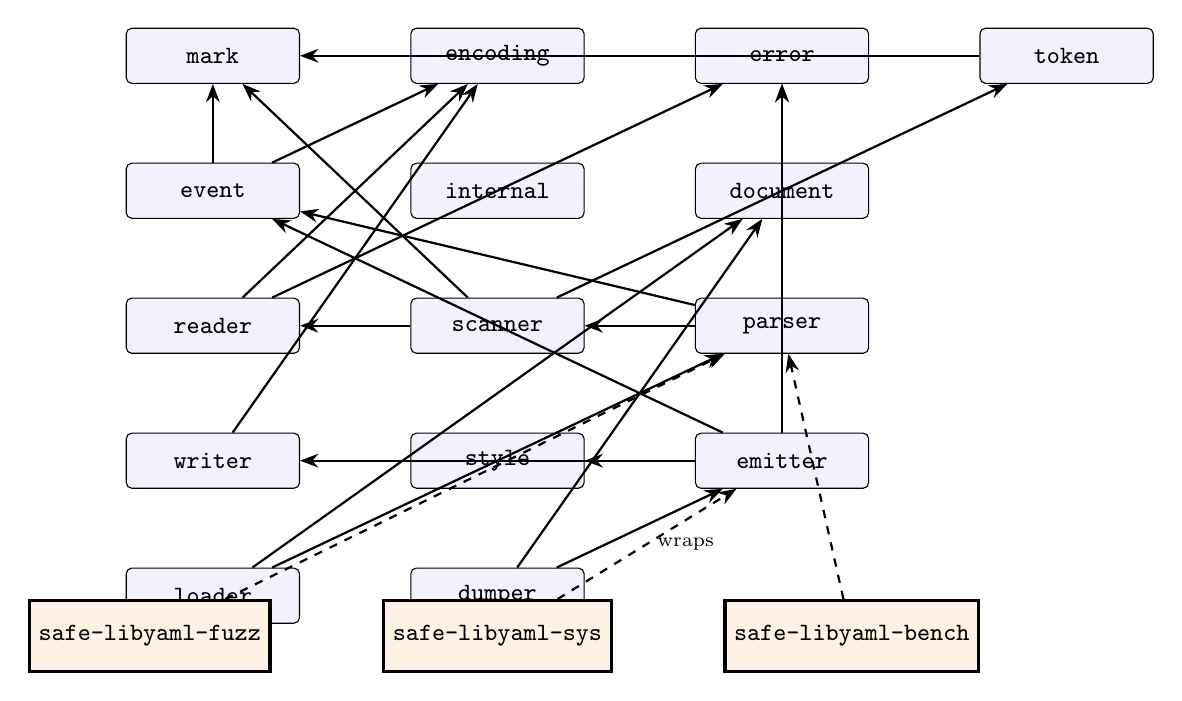
\begin{tikzpicture}[
  node distance=10mm and 14mm,
  every node/.style={font=\small},
  modnode/.style={rectangle, draw, rounded corners=2pt, minimum width=22mm, minimum height=7mm, fill=blue!5},
  cratenode/.style={rectangle, draw, very thick, minimum width=28mm, minimum height=9mm, fill=orange!10},
  arr/.style={-Stealth, thick},
  darr/.style={-Stealth, dashed, thick}
]

% Nodes
\node[modnode] (mark)     {\texttt{mark}};
\node[modnode, right=of mark] (encoding) {\texttt{encoding}};
\node[modnode, right=of encoding] (error)   {\texttt{error}};
\node[modnode, right=of error] (token)    {\texttt{token}};

\node[modnode, below=of mark]      (event)   {\texttt{event}};
\node[modnode, right=of event]     (internal){\texttt{internal}};
\node[modnode, right=of internal]  (document){\texttt{document}};

\node[modnode, below=of event]     (reader) {\texttt{reader}};
\node[modnode, right=of reader]    (scanner){\texttt{scanner}};
\node[modnode, right=of scanner]   (parser) {\texttt{parser}};

\node[modnode, below=of reader]    (writer) {\texttt{writer}};
\node[modnode, right=of writer]    (style)  {\texttt{style}};
\node[modnode, right=of style]     (emitter){\texttt{emitter}};

\node[modnode, below=of writer]    (loader) {\texttt{loader}};
\node[modnode, right=of loader]    (dumper) {\texttt{dumper}};

\node[cratenode, below=14mm of style] (sys) {\texttt{safe-libyaml-sys}};
\node[cratenode, left=of sys]  (fuzz) {\texttt{safe-libyaml-fuzz}};
\node[cratenode, right=of sys] (bench){\texttt{safe-libyaml-bench}};

% Edges
\draw[arr] (event) -- (mark);
\draw[arr] (event) -- (encoding);
\draw[arr] (token) -- (mark);
\draw[arr] (reader) -- (encoding);
\draw[arr] (reader) -- (error);
\draw[arr] (scanner) -- (token);
\draw[arr] (scanner) -- (reader);
\draw[arr] (scanner) -- (mark);
\draw[arr] (parser) -- (scanner);
\draw[arr] (parser) -- (event);
\draw[arr] (parser) -- (error);
\draw[arr] (writer) -- (encoding);
\draw[arr] (emitter) -- (event);
\draw[arr] (emitter) -- (writer);
\draw[arr] (emitter) -- (style);
\draw[arr] (emitter) -- (error);
\draw[arr] (loader) -- (parser);
\draw[arr] (loader) -- (document);
\draw[arr] (dumper) -- (emitter);
\draw[arr] (dumper) -- (document);

\draw[darr] (sys) -- node[midway, right, font=\scriptsize] {wraps} (emitter);
\draw[darr] (fuzz) -- (parser);
\draw[darr] (bench) -- (parser);

\end{tikzpicture}
\end{center}

\noindent\textbf{Reading.} The four ``leaf'' modules (\texttt{mark},
\texttt{encoding}, \texttt{error}, \texttt{token}) have no
\texttt{safe-libyaml}-internal dependencies and are translated first
(Phase B Wave 1). The middle row (\texttt{event}, \texttt{internal},
\texttt{document}) depends only on the leaves. The bottom rows
(\texttt{reader}/\texttt{scanner}/\texttt{parser},
\texttt{writer}/\texttt{style}/\texttt{emitter},
\texttt{loader}/\texttt{dumper}) form the streaming pipeline. The three
sister crates (\texttt{-sys}, \texttt{-fuzz}, \texttt{-bench}) depend on
the safe core but never on each other.

\subsection{Reference \texttt{lints.toml}}

\begin{lstlisting}[language={}]
# safe-libyaml/lints.toml -- consumed by C4 (Idiom Polisher)
[lints.rust]
unsafe_code = "deny"
missing_docs = "deny"
rust_2018_idioms = "deny"

[lints.clippy]
pedantic = { level = "warn", priority = -1 }
nursery  = { level = "warn", priority = -1 }
# Project-specific allows (justify each in PR description)
module_name_repetitions = "allow"
missing_errors_doc      = "allow"   # covered by Error type docs
must_use_candidate      = "warn"
needless_range_loop     = "deny"
\end{lstlisting}

\subsection{Hand-off to Phase B}

The artifacts produced by the agents in this appendix --- the workspace, the
crate skeletons with \texttt{todo!()} bodies, the FFI shim with stub bodies
delegating to the safe crate, and \texttt{cbindgen.toml} producing a
parity header --- form the input contract for Phase B (the per-function
TRANSLATE-TEST-FIX loop) which is described in the companion
\texttt{c-rust-transpiling} paper. Phase B agents replace each
\texttt{todo!()} with a real implementation while preserving every type
signature emitted by the OSG-to-Rust emitter, ensuring the type-contract
discipline mandated by the supervisory \texttt{CLAUDE.md} rules.

\end{document}
